% Options for packages loaded elsewhere
% Options for packages loaded elsewhere
\PassOptionsToPackage{unicode}{hyperref}
\PassOptionsToPackage{hyphens}{url}
\PassOptionsToPackage{dvipsnames,svgnames,x11names}{xcolor}
%
\documentclass[
  letterpaper,
  DIV=11,
  numbers=noendperiod]{scrartcl}
\usepackage{xcolor}
\usepackage{amsmath,amssymb}
\setcounter{secnumdepth}{-\maxdimen} % remove section numbering
\usepackage{iftex}
\ifPDFTeX
  \usepackage[T1]{fontenc}
  \usepackage[utf8]{inputenc}
  \usepackage{textcomp} % provide euro and other symbols
\else % if luatex or xetex
  \usepackage{unicode-math} % this also loads fontspec
  \defaultfontfeatures{Scale=MatchLowercase}
  \defaultfontfeatures[\rmfamily]{Ligatures=TeX,Scale=1}
\fi
\usepackage{lmodern}
\ifPDFTeX\else
  % xetex/luatex font selection
\fi
% Use upquote if available, for straight quotes in verbatim environments
\IfFileExists{upquote.sty}{\usepackage{upquote}}{}
\IfFileExists{microtype.sty}{% use microtype if available
  \usepackage[]{microtype}
  \UseMicrotypeSet[protrusion]{basicmath} % disable protrusion for tt fonts
}{}
\makeatletter
\@ifundefined{KOMAClassName}{% if non-KOMA class
  \IfFileExists{parskip.sty}{%
    \usepackage{parskip}
  }{% else
    \setlength{\parindent}{0pt}
    \setlength{\parskip}{6pt plus 2pt minus 1pt}}
}{% if KOMA class
  \KOMAoptions{parskip=half}}
\makeatother
% Make \paragraph and \subparagraph free-standing
\makeatletter
\ifx\paragraph\undefined\else
  \let\oldparagraph\paragraph
  \renewcommand{\paragraph}{
    \@ifstar
      \xxxParagraphStar
      \xxxParagraphNoStar
  }
  \newcommand{\xxxParagraphStar}[1]{\oldparagraph*{#1}\mbox{}}
  \newcommand{\xxxParagraphNoStar}[1]{\oldparagraph{#1}\mbox{}}
\fi
\ifx\subparagraph\undefined\else
  \let\oldsubparagraph\subparagraph
  \renewcommand{\subparagraph}{
    \@ifstar
      \xxxSubParagraphStar
      \xxxSubParagraphNoStar
  }
  \newcommand{\xxxSubParagraphStar}[1]{\oldsubparagraph*{#1}\mbox{}}
  \newcommand{\xxxSubParagraphNoStar}[1]{\oldsubparagraph{#1}\mbox{}}
\fi
\makeatother


\usepackage{longtable,booktabs,array}
\usepackage{calc} % for calculating minipage widths
% Correct order of tables after \paragraph or \subparagraph
\usepackage{etoolbox}
\makeatletter
\patchcmd\longtable{\par}{\if@noskipsec\mbox{}\fi\par}{}{}
\makeatother
% Allow footnotes in longtable head/foot
\IfFileExists{footnotehyper.sty}{\usepackage{footnotehyper}}{\usepackage{footnote}}
\makesavenoteenv{longtable}
\usepackage{graphicx}
\makeatletter
\newsavebox\pandoc@box
\newcommand*\pandocbounded[1]{% scales image to fit in text height/width
  \sbox\pandoc@box{#1}%
  \Gscale@div\@tempa{\textheight}{\dimexpr\ht\pandoc@box+\dp\pandoc@box\relax}%
  \Gscale@div\@tempb{\linewidth}{\wd\pandoc@box}%
  \ifdim\@tempb\p@<\@tempa\p@\let\@tempa\@tempb\fi% select the smaller of both
  \ifdim\@tempa\p@<\p@\scalebox{\@tempa}{\usebox\pandoc@box}%
  \else\usebox{\pandoc@box}%
  \fi%
}
% Set default figure placement to htbp
\def\fps@figure{htbp}
\makeatother





\setlength{\emergencystretch}{3em} % prevent overfull lines

\providecommand{\tightlist}{%
  \setlength{\itemsep}{0pt}\setlength{\parskip}{0pt}}



 


\KOMAoption{captions}{tableheading}
\makeatletter
\@ifpackageloaded{caption}{}{\usepackage{caption}}
\AtBeginDocument{%
\ifdefined\contentsname
  \renewcommand*\contentsname{Table of contents}
\else
  \newcommand\contentsname{Table of contents}
\fi
\ifdefined\listfigurename
  \renewcommand*\listfigurename{List of Figures}
\else
  \newcommand\listfigurename{List of Figures}
\fi
\ifdefined\listtablename
  \renewcommand*\listtablename{List of Tables}
\else
  \newcommand\listtablename{List of Tables}
\fi
\ifdefined\figurename
  \renewcommand*\figurename{Figure}
\else
  \newcommand\figurename{Figure}
\fi
\ifdefined\tablename
  \renewcommand*\tablename{Table}
\else
  \newcommand\tablename{Table}
\fi
}
\@ifpackageloaded{float}{}{\usepackage{float}}
\floatstyle{ruled}
\@ifundefined{c@chapter}{\newfloat{codelisting}{h}{lop}}{\newfloat{codelisting}{h}{lop}[chapter]}
\floatname{codelisting}{Listing}
\newcommand*\listoflistings{\listof{codelisting}{List of Listings}}
\makeatother
\makeatletter
\makeatother
\makeatletter
\@ifpackageloaded{caption}{}{\usepackage{caption}}
\@ifpackageloaded{subcaption}{}{\usepackage{subcaption}}
\makeatother
\usepackage{bookmark}
\IfFileExists{xurl.sty}{\usepackage{xurl}}{} % add URL line breaks if available
\urlstyle{same}
\hypersetup{
  pdftitle={DAMA-DMBOK Framework},
  colorlinks=true,
  linkcolor={blue},
  filecolor={Maroon},
  citecolor={Blue},
  urlcolor={Blue},
  pdfcreator={LaTeX via pandoc}}


\title{DAMA-DMBOK Framework}
\author{}
\date{}
\begin{document}
\maketitle


\section{1. Overview}\label{overview}

\subsection{1.1 Framework Summary}\label{framework-summary}

\begin{longtable}[]{@{}ll@{}}
\toprule\noalign{}
Attribute & Description \\
\midrule\noalign{}
\endhead
\bottomrule\noalign{}
\endlastfoot
Framework Name & DAMA-DMBOK \\
Full Name & Data Management Body of Knowledge \\
Publisher & DAMA International \\
Framework Type & Body of Knowledge \\
Primary Domain & Data Management and Data Governance \\
Primary Focus & Managing data as a strategic enterprise asset \\
Typical Scope & Enterprise-wide \\
Nature & Guidance, principles, practices, and capability model \\
\end{longtable}

\subsection{1.2 DAMA and DMBOK}\label{dama-and-dmbok}

DAMA International is the professional association that promotes the
discipline of data management.\\
DMBOK is the body of knowledge published by DAMA and used as the main
reference model for enterprise data management.

For consistency with the wider enterprise governance book, this chapter
treats \textbf{DMBOK} as the framework and \textbf{DAMA} as the
organisational and professional context around it.

\subsection{1.3 Purpose}\label{purpose}

DMBOK provides a structured view of the disciplines required to manage
data across its lifecycle. It helps organisations treat data as a
strategic asset by establishing governance, architecture, quality,
security, metadata, master data, and analytics capabilities.

\subsection{1.4 Why It Matters}\label{why-it-matters}

DMBOK is particularly valuable where organisations need to:

\begin{itemize}
\tightlist
\item
  establish enterprise data governance
\item
  improve trust in data
\item
  reduce duplication and inconsistency
\item
  strengthen compliance and control
\item
  support analytics, reporting, and AI
\item
  align business, technology, and risk perspectives around data
\end{itemize}

\section{2. Core Principles}\label{core-principles}

DMBOK is underpinned by a small set of core ideas that remain useful
across sectors and operating models.

\begin{itemize}
\tightlist
\item
  Data is an enterprise asset.
\item
  Data must be governed.
\item
  Data management spans the full lifecycle.
\item
  Data quality, security, and ethics are essential.
\item
  Metadata is foundational.
\item
  Data management requires business and technical collaboration.
\item
  Accountability and stewardship are necessary to sustain control and
  value.
\end{itemize}

\section{3. Knowledge Areas}\label{knowledge-areas}

\subsection{3.1 DMBOK Knowledge Areas}\label{dmbok-knowledge-areas}

\begin{longtable}[]{@{}
  >{\raggedright\arraybackslash}p{(\linewidth - 4\tabcolsep) * \real{0.3333}}
  >{\raggedright\arraybackslash}p{(\linewidth - 4\tabcolsep) * \real{0.3333}}
  >{\raggedright\arraybackslash}p{(\linewidth - 4\tabcolsep) * \real{0.3333}}@{}}
\toprule\noalign{}
\begin{minipage}[b]{\linewidth}\raggedright
\#
\end{minipage} & \begin{minipage}[b]{\linewidth}\raggedright
Knowledge Area
\end{minipage} & \begin{minipage}[b]{\linewidth}\raggedright
Description
\end{minipage} \\
\midrule\noalign{}
\endhead
\bottomrule\noalign{}
\endlastfoot
1 & Data Governance & Policies, standards, decision rights,
accountability \\
2 & Data Architecture & Structure, principles, integration, and target
state \\
3 & Data Modelling and Design & Conceptual, logical, and physical data
models \\
4 & Data Storage and Operations & Databases, storage, backup, recovery,
operational handling \\
5 & Data Security & Protection, privacy, access, classification, and
control \\
6 & Data Integration and Interoperability & ETL, APIs, messaging,
interfaces, and exchange \\
7 & Document and Content Management & Unstructured information and
content handling \\
8 & Reference and Master Data & Shared definitions, golden records,
consistency \\
9 & Data Warehousing and Business Intelligence & Reporting, analytics,
and decision support \\
10 & Metadata Management & Business definitions, lineage,
classification, and context \\
11 & Data Quality & Accuracy, completeness, consistency, and fitness for
use \\
\end{longtable}

\subsection{3.2 Knowledge Areas Map}\label{knowledge-areas-map}

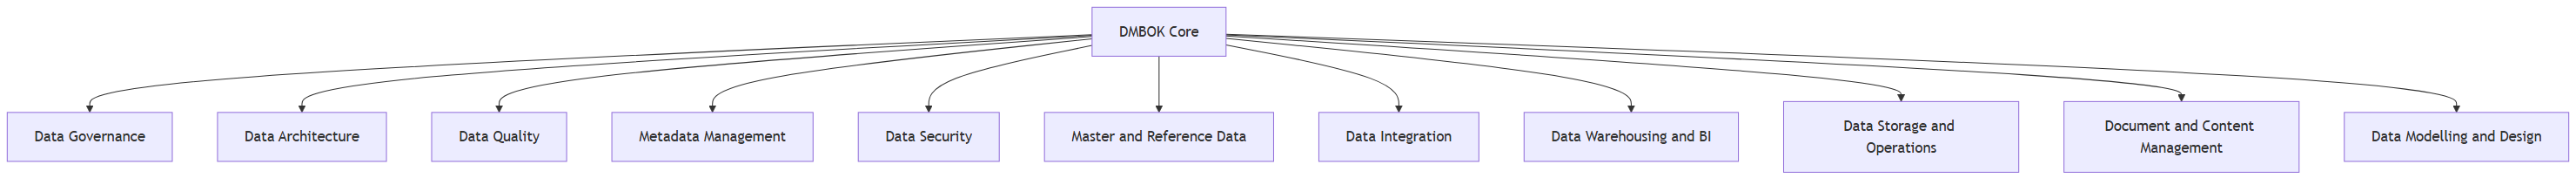
\includegraphics[width=29.67in,height=2.06in]{dama_dmbok_cobit_style_v2_files/figure-latex/mermaid-figure-1.png}

\section{4. Process Structure}\label{process-structure}

\subsection{4.1 Generic Operating
Pattern}\label{generic-operating-pattern}

Unlike COBIT, DMBOK is not primarily organised as a numbered process
catalogue. However, its knowledge areas can be applied through a
consistent operating pattern.

\begin{longtable}[]{@{}
  >{\raggedright\arraybackslash}p{(\linewidth - 2\tabcolsep) * \real{0.5000}}
  >{\raggedright\arraybackslash}p{(\linewidth - 2\tabcolsep) * \real{0.5000}}@{}}
\toprule\noalign{}
\begin{minipage}[b]{\linewidth}\raggedright
Element
\end{minipage} & \begin{minipage}[b]{\linewidth}\raggedright
Description
\end{minipage} \\
\midrule\noalign{}
\endhead
\bottomrule\noalign{}
\endlastfoot
Inputs & Business strategy, regulatory obligations, data needs,
policies, source systems \\
Activities & Define, design, implement, monitor, improve \\
Outputs & Policies, models, standards, controls, metadata, reports,
governed data assets \\
\end{longtable}

\subsection{4.2 Inputs → Processes → Outputs →
Consumers}\label{inputs-processes-outputs-consumers}

\subsubsection{Data Governance Example}\label{data-governance-example}

\begin{longtable}[]{@{}
  >{\raggedright\arraybackslash}p{(\linewidth - 2\tabcolsep) * \real{0.5000}}
  >{\raggedright\arraybackslash}p{(\linewidth - 2\tabcolsep) * \real{0.5000}}@{}}
\toprule\noalign{}
\begin{minipage}[b]{\linewidth}\raggedright
Element
\end{minipage} & \begin{minipage}[b]{\linewidth}\raggedright
Description
\end{minipage} \\
\midrule\noalign{}
\endhead
\bottomrule\noalign{}
\endlastfoot
Inputs & Strategy, regulation, risk requirements, operating model \\
Processes & Define policies, assign ownership, establish stewardship,
govern priorities \\
Outputs & Data strategy, governance framework, policies, standards,
ownership model \\
Consumers & Business units, IT, risk, compliance, projects,
operations \\
\end{longtable}

\subsubsection{Data Quality Example}\label{data-quality-example}

\begin{longtable}[]{@{}
  >{\raggedright\arraybackslash}p{(\linewidth - 2\tabcolsep) * \real{0.5000}}
  >{\raggedright\arraybackslash}p{(\linewidth - 2\tabcolsep) * \real{0.5000}}@{}}
\toprule\noalign{}
\begin{minipage}[b]{\linewidth}\raggedright
Element
\end{minipage} & \begin{minipage}[b]{\linewidth}\raggedright
Description
\end{minipage} \\
\midrule\noalign{}
\endhead
\bottomrule\noalign{}
\endlastfoot
Inputs & Critical data sets, business rules, quality thresholds \\
Processes & Profile, validate, monitor, correct, improve \\
Outputs & Quality rules, issue log, quality metrics, quality reports \\
Consumers & Operations, analytics teams, business owners, governance
forums \\
\end{longtable}

\subsubsection{Metadata Management
Example}\label{metadata-management-example}

\begin{longtable}[]{@{}
  >{\raggedright\arraybackslash}p{(\linewidth - 2\tabcolsep) * \real{0.5000}}
  >{\raggedright\arraybackslash}p{(\linewidth - 2\tabcolsep) * \real{0.5000}}@{}}
\toprule\noalign{}
\begin{minipage}[b]{\linewidth}\raggedright
Element
\end{minipage} & \begin{minipage}[b]{\linewidth}\raggedright
Description
\end{minipage} \\
\midrule\noalign{}
\endhead
\bottomrule\noalign{}
\endlastfoot
Inputs & Source systems, data models, integration flows, business
terms \\
Processes & Capture, classify, catalogue, trace lineage, publish
definitions \\
Outputs & Metadata catalogue, business glossary, lineage model,
classification model \\
Consumers & Business users, architects, engineers, audit, security \\
\end{longtable}

\section{5. DAMA Ecosystem Context}\label{dama-ecosystem-context}

\subsection{5.1 DAMA Ecosystem}\label{dama-ecosystem}

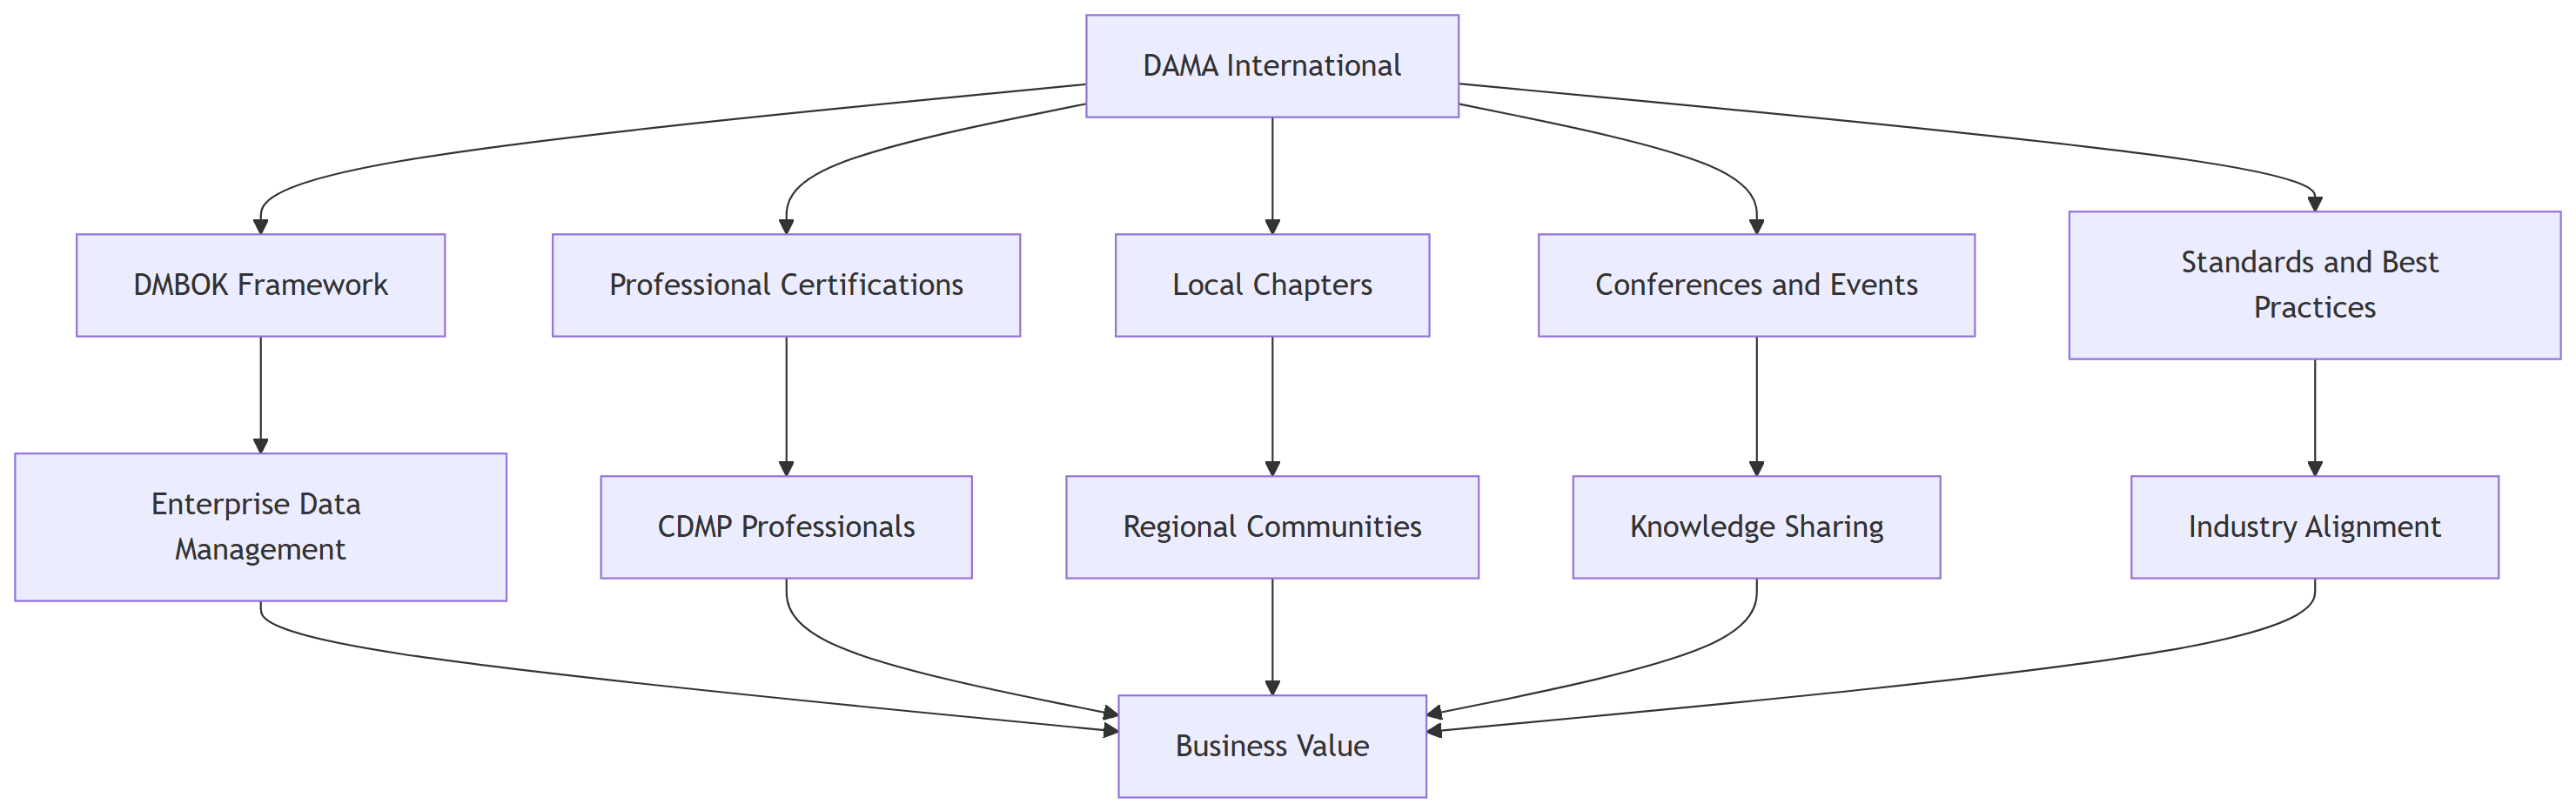
\includegraphics[width=14.2in,height=4.48in]{dama_dmbok_cobit_style_v2_files/figure-latex/mermaid-figure-16.png}

\subsection{5.2 Certification Model}\label{certification-model}

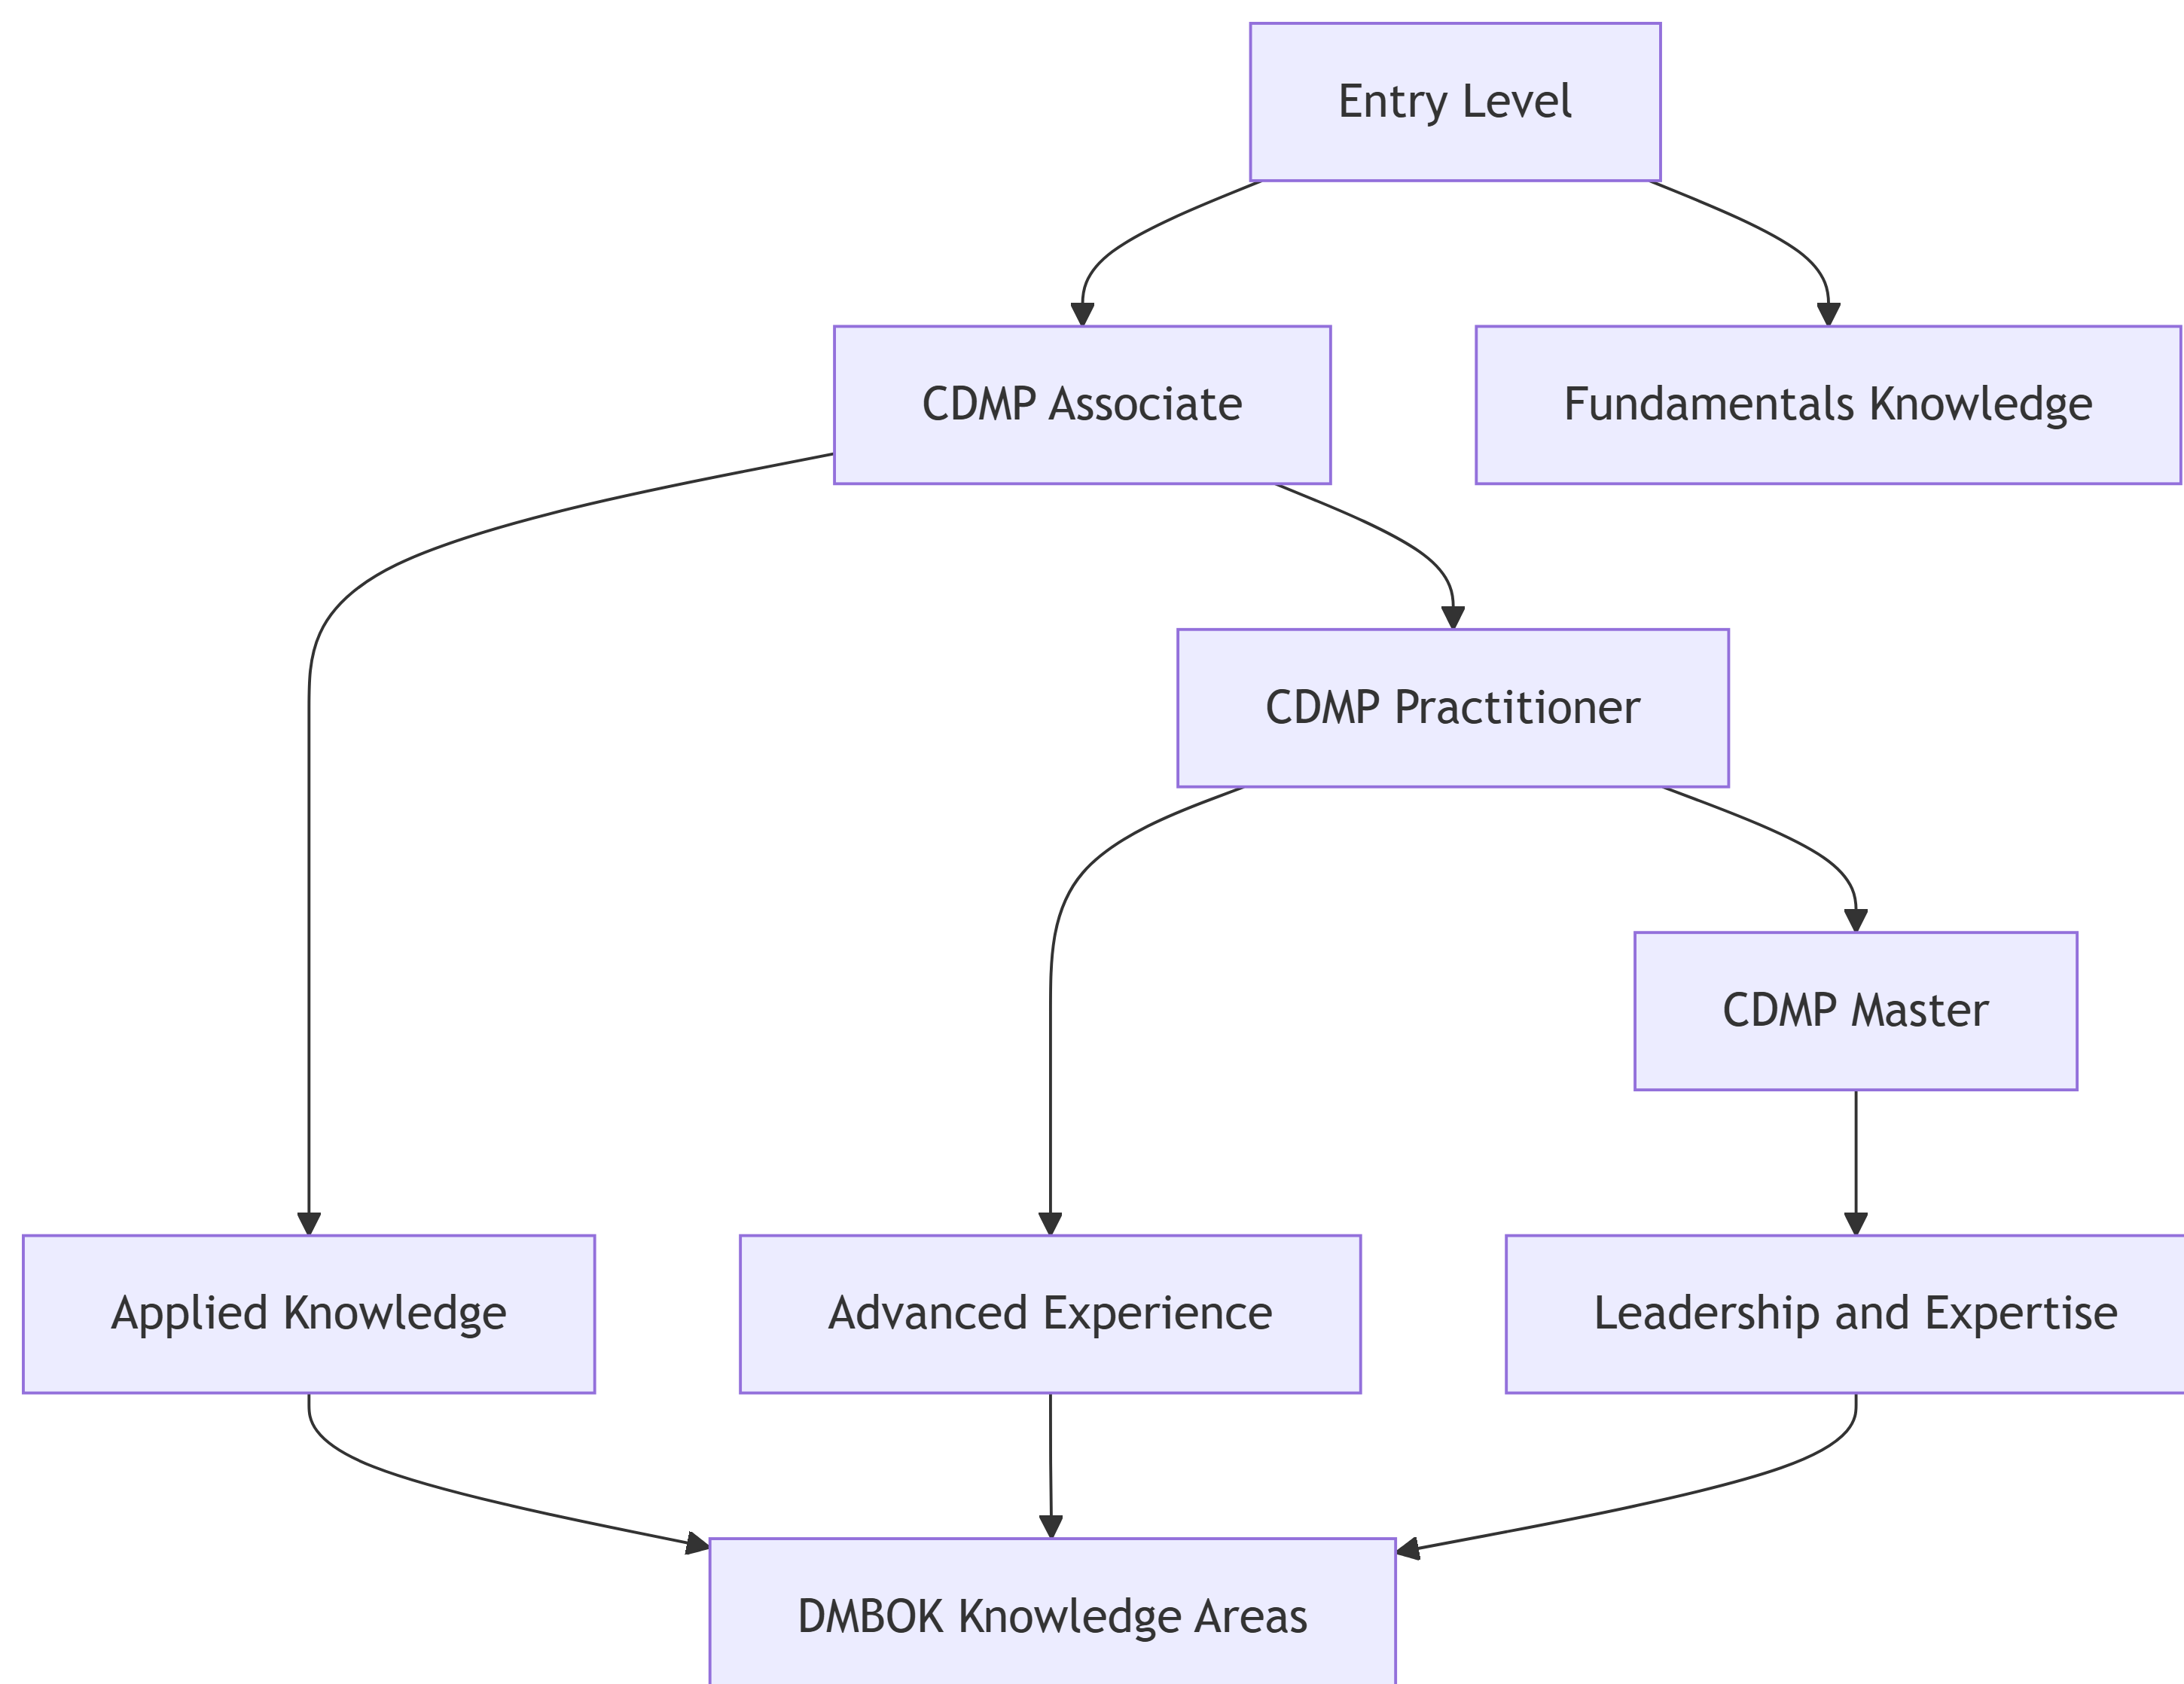
\includegraphics[width=7.97in,height=6.15in]{dama_dmbok_cobit_style_v2_files/figure-latex/mermaid-figure-15.png}

\section{6. Enterprise Data Management
View}\label{enterprise-data-management-view}

\subsection{6.1 Capability Overview}\label{capability-overview}

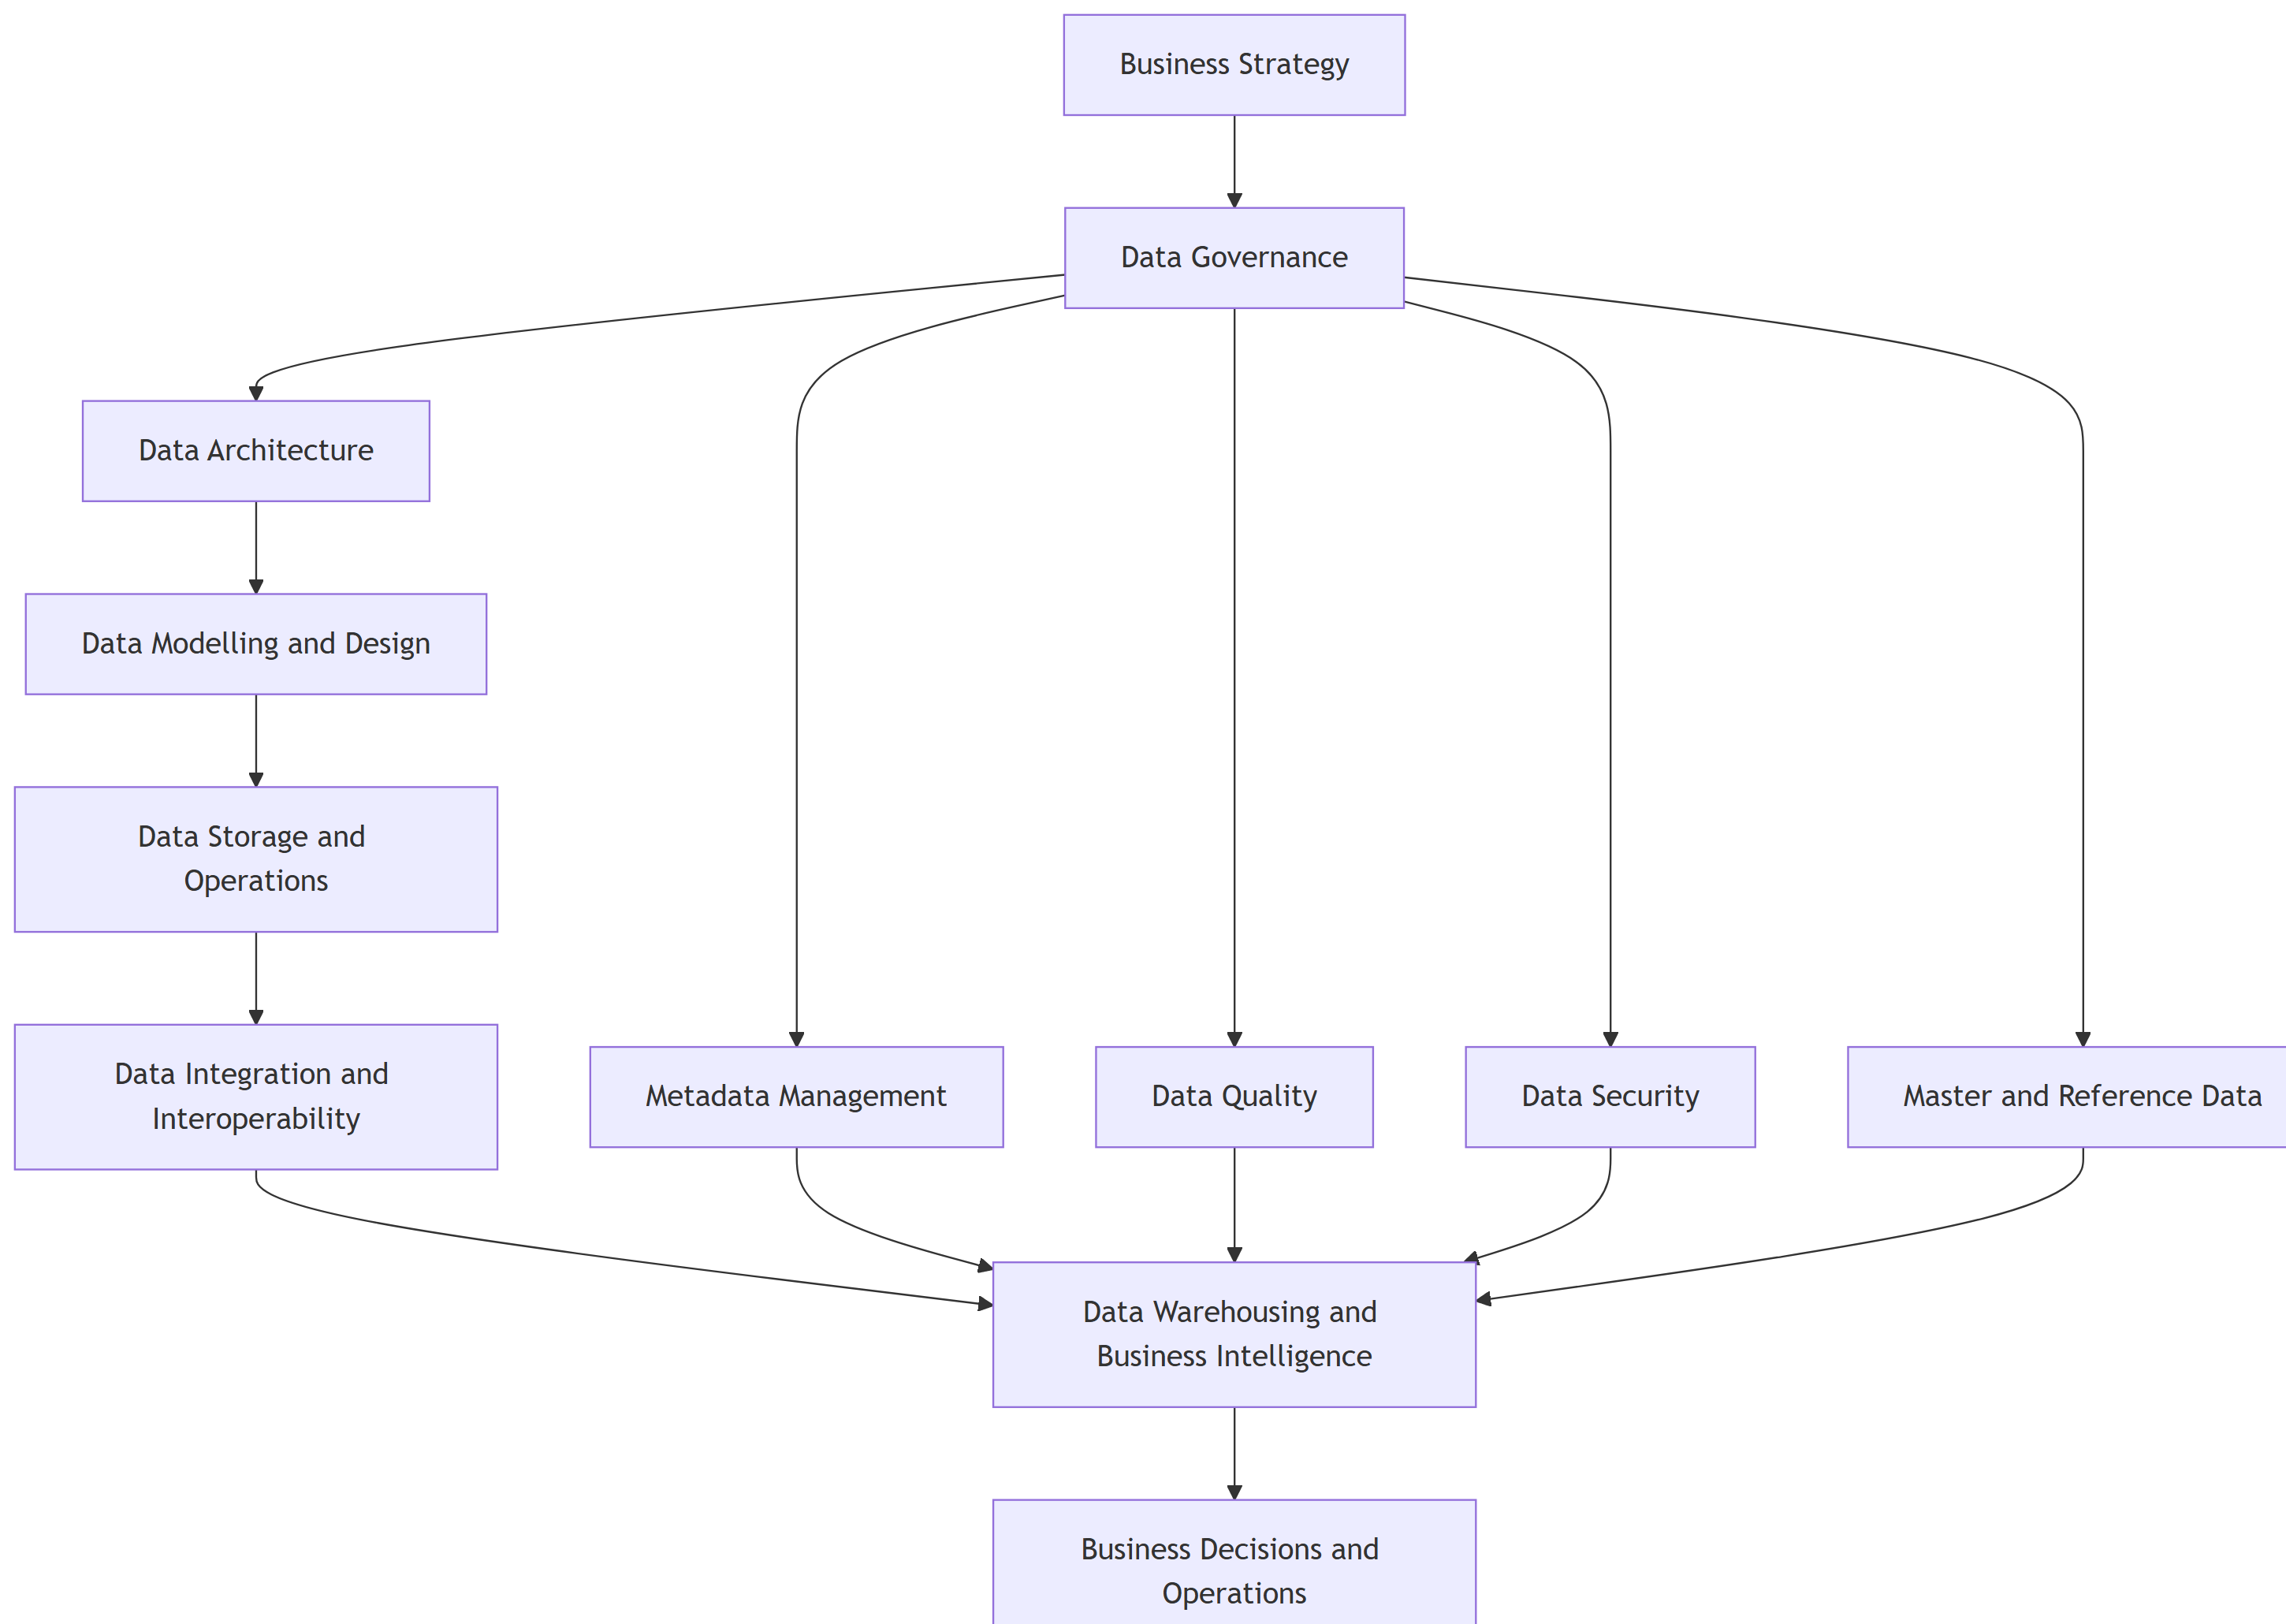
\includegraphics[width=13.09in,height=9.31in]{dama_dmbok_cobit_style_v2_files/figure-latex/mermaid-figure-14.png}

\subsection{6.2 Knowledge Areas Interaction
Map}\label{knowledge-areas-interaction-map}

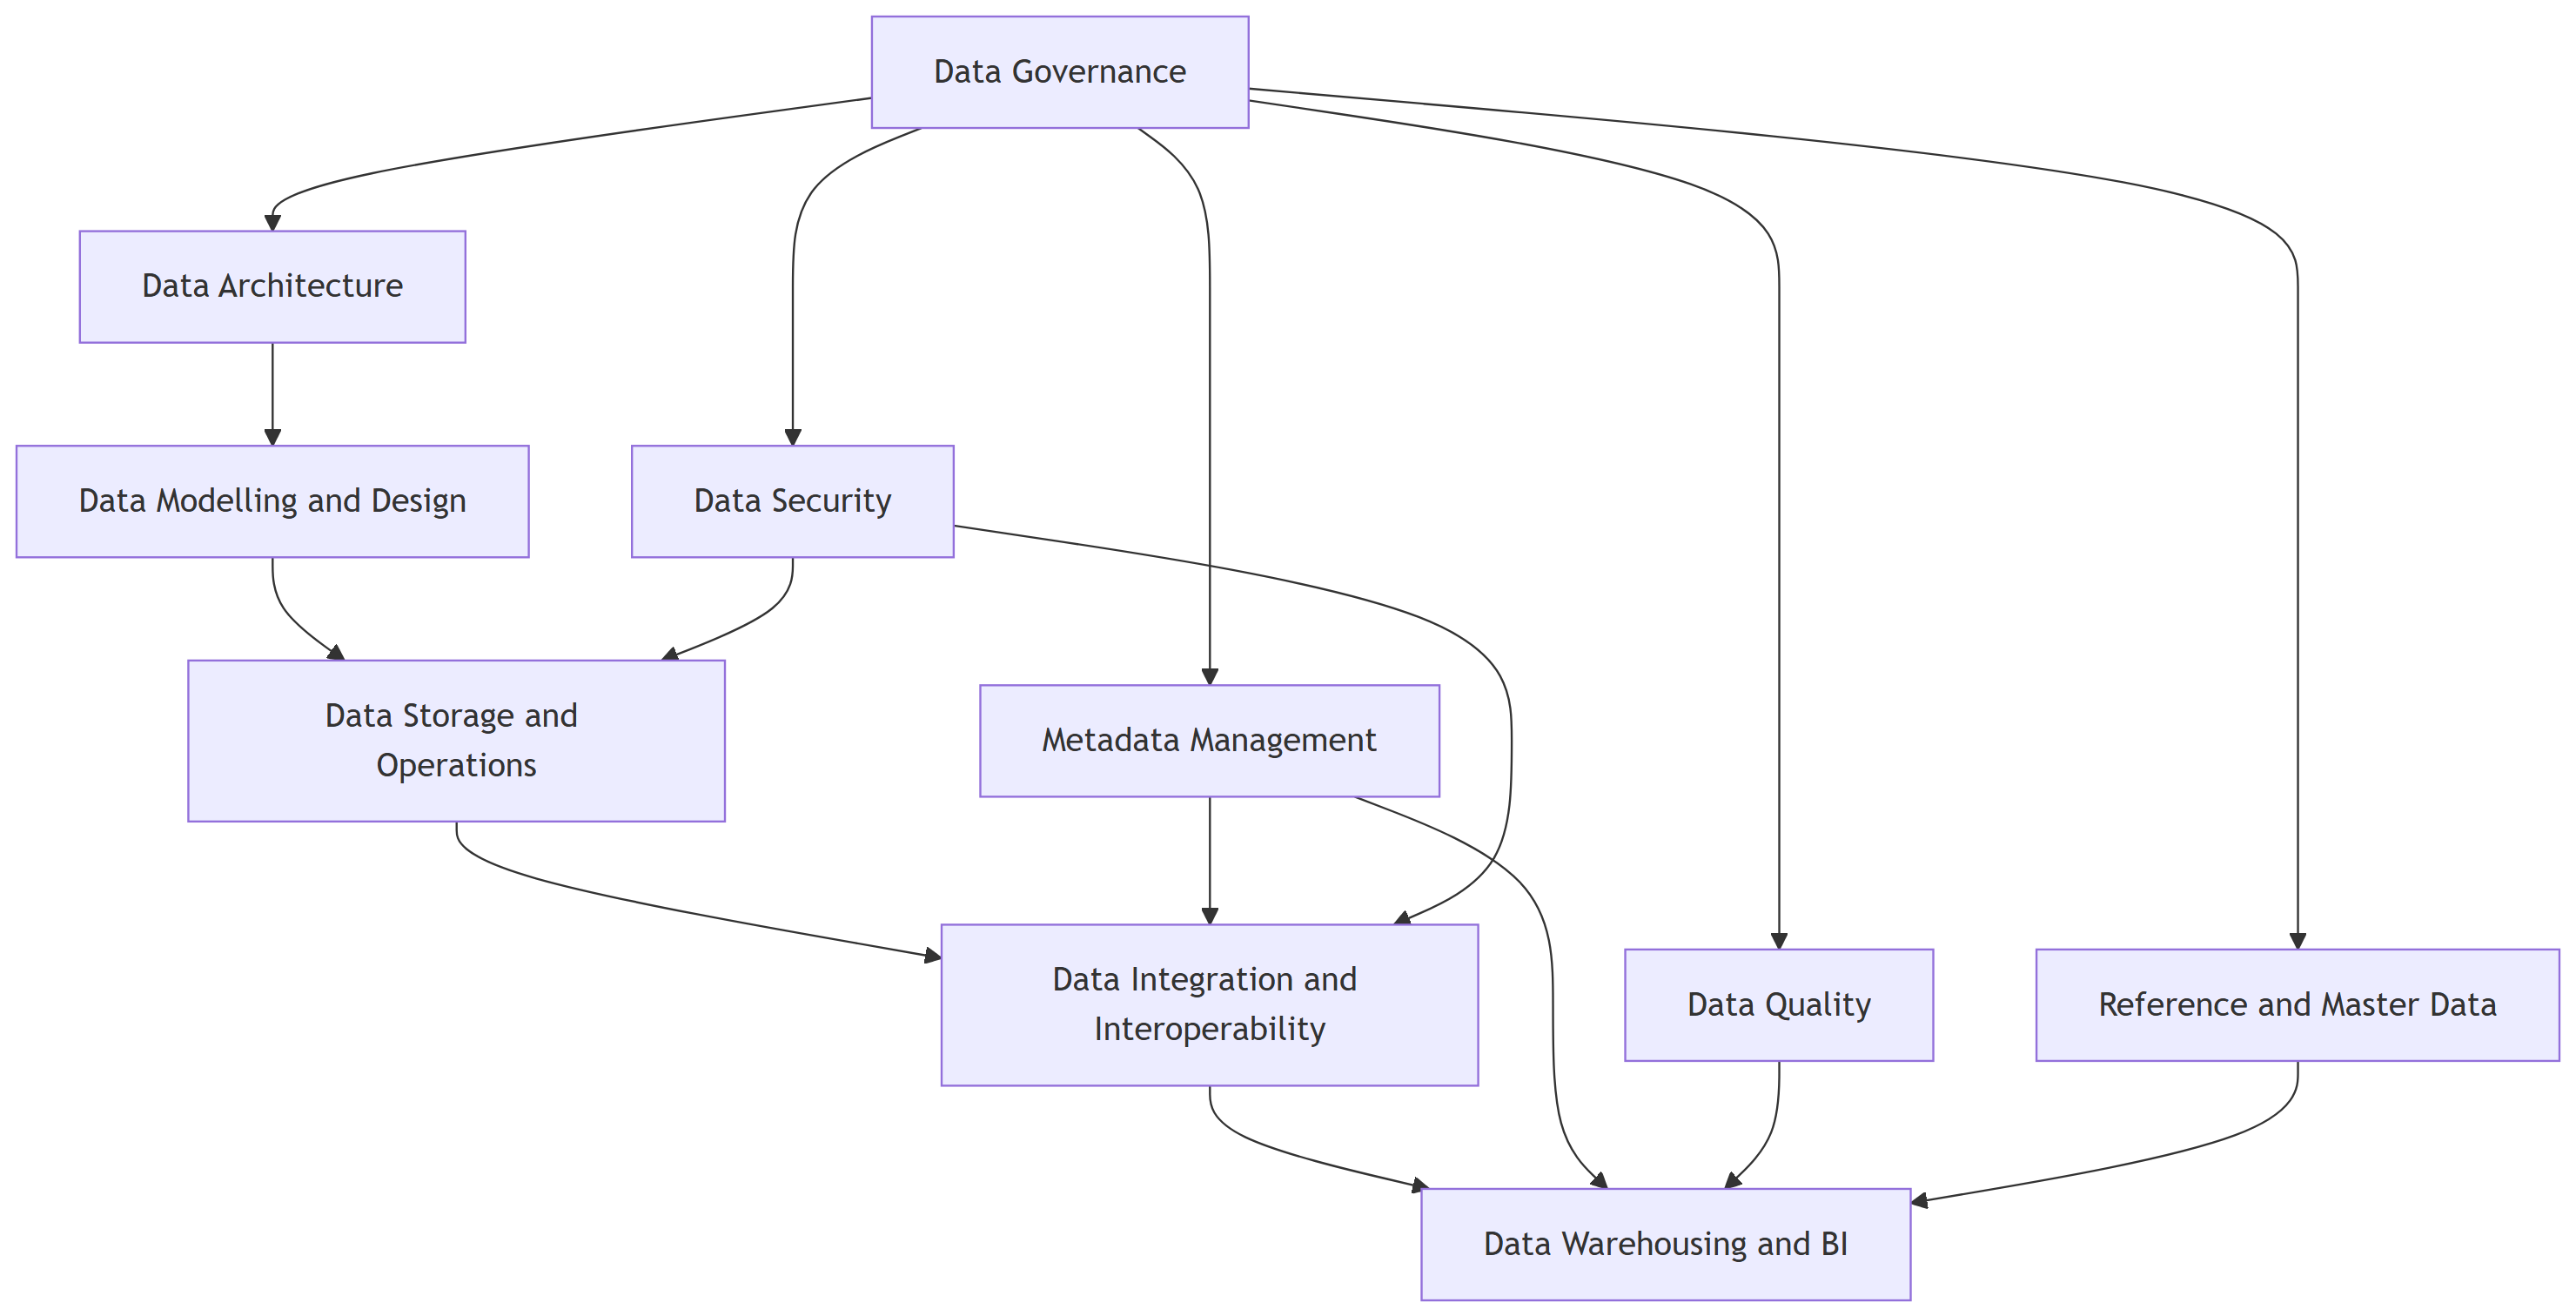
\includegraphics[width=13in,height=6.65in]{dama_dmbok_cobit_style_v2_files/figure-latex/mermaid-figure-13.png}

\section{7. Lifecycle View}\label{lifecycle-view}

\subsection{7.1 Data Lifecycle}\label{data-lifecycle}

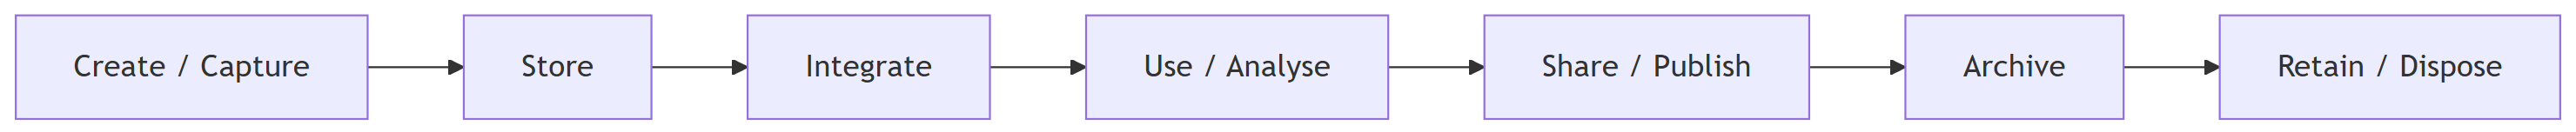
\includegraphics[width=13.95in,height=0.73in]{dama_dmbok_cobit_style_v2_files/figure-latex/mermaid-figure-12.png}

\subsection{7.2 Lifecycle Mapping to
DMBOK}\label{lifecycle-mapping-to-dmbok}

\begin{longtable}[]{@{}
  >{\raggedright\arraybackslash}p{(\linewidth - 2\tabcolsep) * \real{0.5000}}
  >{\raggedright\arraybackslash}p{(\linewidth - 2\tabcolsep) * \real{0.5000}}@{}}
\toprule\noalign{}
\begin{minipage}[b]{\linewidth}\raggedright
Lifecycle Stage
\end{minipage} & \begin{minipage}[b]{\linewidth}\raggedright
Primary DMBOK Areas
\end{minipage} \\
\midrule\noalign{}
\endhead
\bottomrule\noalign{}
\endlastfoot
Create / Capture & Data Modelling and Design, Data Governance \\
Store & Data Storage and Operations, Data Security \\
Integrate & Data Integration and Interoperability, Metadata
Management \\
Use / Analyse & Data Warehousing and BI, Master and Reference Data \\
Share / Publish & Metadata Management, Data Security \\
Archive & Document and Content Management, Governance \\
Retain / Dispose & Governance, Security, Privacy, Compliance \\
\end{longtable}

\section{8. Roles and
Responsibilities}\label{roles-and-responsibilities}

\subsection{8.1 Key Roles}\label{key-roles}

\begin{longtable}[]{@{}
  >{\raggedright\arraybackslash}p{(\linewidth - 2\tabcolsep) * \real{0.5000}}
  >{\raggedright\arraybackslash}p{(\linewidth - 2\tabcolsep) * \real{0.5000}}@{}}
\toprule\noalign{}
\begin{minipage}[b]{\linewidth}\raggedright
Role
\end{minipage} & \begin{minipage}[b]{\linewidth}\raggedright
Responsibility
\end{minipage} \\
\midrule\noalign{}
\endhead
\bottomrule\noalign{}
\endlastfoot
Chief Data Officer (CDO) & Enterprise accountability for data strategy
and governance \\
Data Owner & Accountability for a business data domain \\
Data Steward & Day-to-day governance, quality, and definition
management \\
Data Architect & Design of enterprise data structures and integration
patterns \\
Data Engineer & Implementation of pipelines, platforms, and
transformations \\
Data Custodian & Technical custody, operations, backup, recovery, and
handling \\
Data Quality Analyst & Quality profiling, monitoring, and issue
analysis \\
Security and Compliance Lead & Privacy, classification, access, and
regulatory control \\
\end{longtable}

\subsection{8.2 RACI Matrix by Knowledge
Area}\label{raci-matrix-by-knowledge-area}

\begin{longtable}[]{@{}
  >{\raggedright\arraybackslash}p{(\linewidth - 16\tabcolsep) * \real{0.1111}}
  >{\raggedright\arraybackslash}p{(\linewidth - 16\tabcolsep) * \real{0.1111}}
  >{\raggedright\arraybackslash}p{(\linewidth - 16\tabcolsep) * \real{0.1111}}
  >{\raggedright\arraybackslash}p{(\linewidth - 16\tabcolsep) * \real{0.1111}}
  >{\raggedright\arraybackslash}p{(\linewidth - 16\tabcolsep) * \real{0.1111}}
  >{\raggedright\arraybackslash}p{(\linewidth - 16\tabcolsep) * \real{0.1111}}
  >{\raggedright\arraybackslash}p{(\linewidth - 16\tabcolsep) * \real{0.1111}}
  >{\raggedright\arraybackslash}p{(\linewidth - 16\tabcolsep) * \real{0.1111}}
  >{\raggedright\arraybackslash}p{(\linewidth - 16\tabcolsep) * \real{0.1111}}@{}}
\toprule\noalign{}
\begin{minipage}[b]{\linewidth}\raggedright
Knowledge Area
\end{minipage} & \begin{minipage}[b]{\linewidth}\raggedright
CDO
\end{minipage} & \begin{minipage}[b]{\linewidth}\raggedright
DO
\end{minipage} & \begin{minipage}[b]{\linewidth}\raggedright
DS
\end{minipage} & \begin{minipage}[b]{\linewidth}\raggedright
DA
\end{minipage} & \begin{minipage}[b]{\linewidth}\raggedright
DE
\end{minipage} & \begin{minipage}[b]{\linewidth}\raggedright
DC
\end{minipage} & \begin{minipage}[b]{\linewidth}\raggedright
DQ
\end{minipage} & \begin{minipage}[b]{\linewidth}\raggedright
SEC
\end{minipage} \\
\midrule\noalign{}
\endhead
\bottomrule\noalign{}
\endlastfoot
Data Governance & A & R & R & C & I & I & C & C \\
Data Architecture & A & C & C & R & C & I & I & C \\
Data Modelling and Design & C & C & R & A & R & I & I & I \\
Data Storage and Operations & I & I & C & C & R & A & I & C \\
Data Security & A & C & C & C & I & R & I & R \\
Data Integration and Interoperability & C & I & C & A & R & C & I & I \\
Document and Content Management & C & R & R & I & I & A & C & C \\
Reference and Master Data & A & R & R & C & C & I & C & I \\
Data Warehousing and BI & C & R & C & A & R & I & C & I \\
Metadata Management & A & C & R & R & C & I & C & I \\
Data Quality & A & R & R & C & C & I & A & I \\
\end{longtable}

\section{9. Key Artefacts}\label{key-artefacts}

\subsection{9.1 Core Artefact Catalogue}\label{core-artefact-catalogue}

\begin{longtable}[]{@{}
  >{\raggedright\arraybackslash}p{(\linewidth - 4\tabcolsep) * \real{0.3333}}
  >{\raggedright\arraybackslash}p{(\linewidth - 4\tabcolsep) * \real{0.3333}}
  >{\raggedright\arraybackslash}p{(\linewidth - 4\tabcolsep) * \real{0.3333}}@{}}
\toprule\noalign{}
\begin{minipage}[b]{\linewidth}\raggedright
Artefact
\end{minipage} & \begin{minipage}[b]{\linewidth}\raggedright
Description
\end{minipage} & \begin{minipage}[b]{\linewidth}\raggedright
Produced By
\end{minipage} \\
\midrule\noalign{}
\endhead
\bottomrule\noalign{}
\endlastfoot
Data Strategy & Enterprise direction, priorities, and goals for data &
Data Governance \\
Data Governance Framework & Decision rights, ownership, forums, and
control model & Data Governance \\
Data Policies and Standards & Rules, controls, definitions, and minimum
requirements & Data Governance \\
Data Architecture Blueprint & Target structure of data and integration
across the estate & Data Architecture \\
Data Models & Conceptual, logical, and physical representations & Data
Modelling and Design \\
Data Dictionary & Standard definitions of key data elements & Metadata
Management \\
Metadata Catalogue & Definitions, lineage, classification, ownership &
Metadata Management \\
Data Lineage Model & End-to-end traceability of data movement and
transformation & Metadata / Integration \\
Data Quality Rules & Rules and validation conditions for critical data &
Data Quality \\
Data Quality Report & Monitoring outputs, trends, and issue positions &
Data Quality \\
Master Data Definitions & Standard entity definitions and ownership
rules & Master and Reference Data \\
Golden Record & Authoritative version of a mastered entity & Master
Data \\
Data Security Policy & Security, access, privacy, and handling
requirements & Data Security \\
Access Control Matrix & Role-based access and segregation rules & Data
Security \\
Integration Specifications & Definitions of interface, pipeline, and
exchange design & Data Integration \\
ETL / Pipeline Definitions & Transformation logic and operational
movement rules & Data Integration \\
BI Reports and Dashboards & Curated outputs for monitoring and
decision-making & Data Warehousing and BI \\
Data Issue Log & Managed record of data issues and remediation actions &
Data Quality \\
Data Retention Policy & Rules for archive, retention, and disposal &
Governance / Security \\
\end{longtable}

\subsection{9.2 Artefact Mapping}\label{artefact-mapping}

\begin{longtable}[]{@{}
  >{\raggedright\arraybackslash}p{(\linewidth - 8\tabcolsep) * \real{0.2000}}
  >{\raggedright\arraybackslash}p{(\linewidth - 8\tabcolsep) * \real{0.2000}}
  >{\raggedright\arraybackslash}p{(\linewidth - 8\tabcolsep) * \real{0.2000}}
  >{\raggedright\arraybackslash}p{(\linewidth - 8\tabcolsep) * \real{0.2000}}
  >{\raggedright\arraybackslash}p{(\linewidth - 8\tabcolsep) * \real{0.2000}}@{}}
\toprule\noalign{}
\begin{minipage}[b]{\linewidth}\raggedright
Artefact
\end{minipage} & \begin{minipage}[b]{\linewidth}\raggedright
Produced By
\end{minipage} & \begin{minipage}[b]{\linewidth}\raggedright
RACI (A / R)
\end{minipage} & \begin{minipage}[b]{\linewidth}\raggedright
Input From
\end{minipage} & \begin{minipage}[b]{\linewidth}\raggedright
Output To
\end{minipage} \\
\midrule\noalign{}
\endhead
\bottomrule\noalign{}
\endlastfoot
Data Strategy & Data Governance & A: CDO / R: DO & Business Strategy &
All Domains \\
Data Governance Framework & Governance & A: CDO / R: DS & Strategy,
Compliance & All Knowledge Areas \\
Data Policies and Standards & Governance & A: CDO / R: DS & Regulatory,
Risk & Architecture, Operations \\
Data Architecture Blueprint & Architecture & A: DA / R: DA & Governance
& Engineering \\
Data Models & Modelling & A: DA / R: DE & Architecture & Storage,
Integration \\
Data Dictionary & Metadata & A: DS / R: DS & Models & Business, IT \\
Metadata Catalogue & Metadata & A: CDO / R: DS & All Systems & All
Users \\
Data Lineage & Metadata & A: DA / R: DE & Integration Flows & Audit,
Risk \\
Data Quality Rules & Quality & A: DQ / R: DS & Business Rules &
Operations \\
Data Quality Reports & Quality & A: DQ / R: DQ & Monitoring &
Governance \\
Master Data Definitions & Master Data & A: DO / R: DS & Business Domains
& All Systems \\
Golden Record & Master Data & A: DO / R: DE & Source Systems &
Consumers \\
Data Security Policy & Security & A: SEC / R: SEC & Risk, Compliance &
IT, Business \\
Access Control Matrix & Security & A: SEC / R: DC & Policies &
Systems \\
Data Integration Specifications & Integration & A: DA / R: DE & Models &
Engineering \\
ETL / Pipeline Definitions & Integration & A: DE / R: DE &
Specifications & Platforms \\
BI Reports and Dashboards & BI & A: DO / R: DE & Data Warehouse &
Business \\
Data Issue Log & Quality & A: DQ / R: DS & Monitoring & Governance \\
Data Retention Policy & Governance & A: SEC / R: CDO & Legal &
Operations \\
\end{longtable}

\section{10. Operating Process
Diagrams}\label{operating-process-diagrams}

\subsection{10.1 Data Quality Management
Cycle}\label{data-quality-management-cycle}

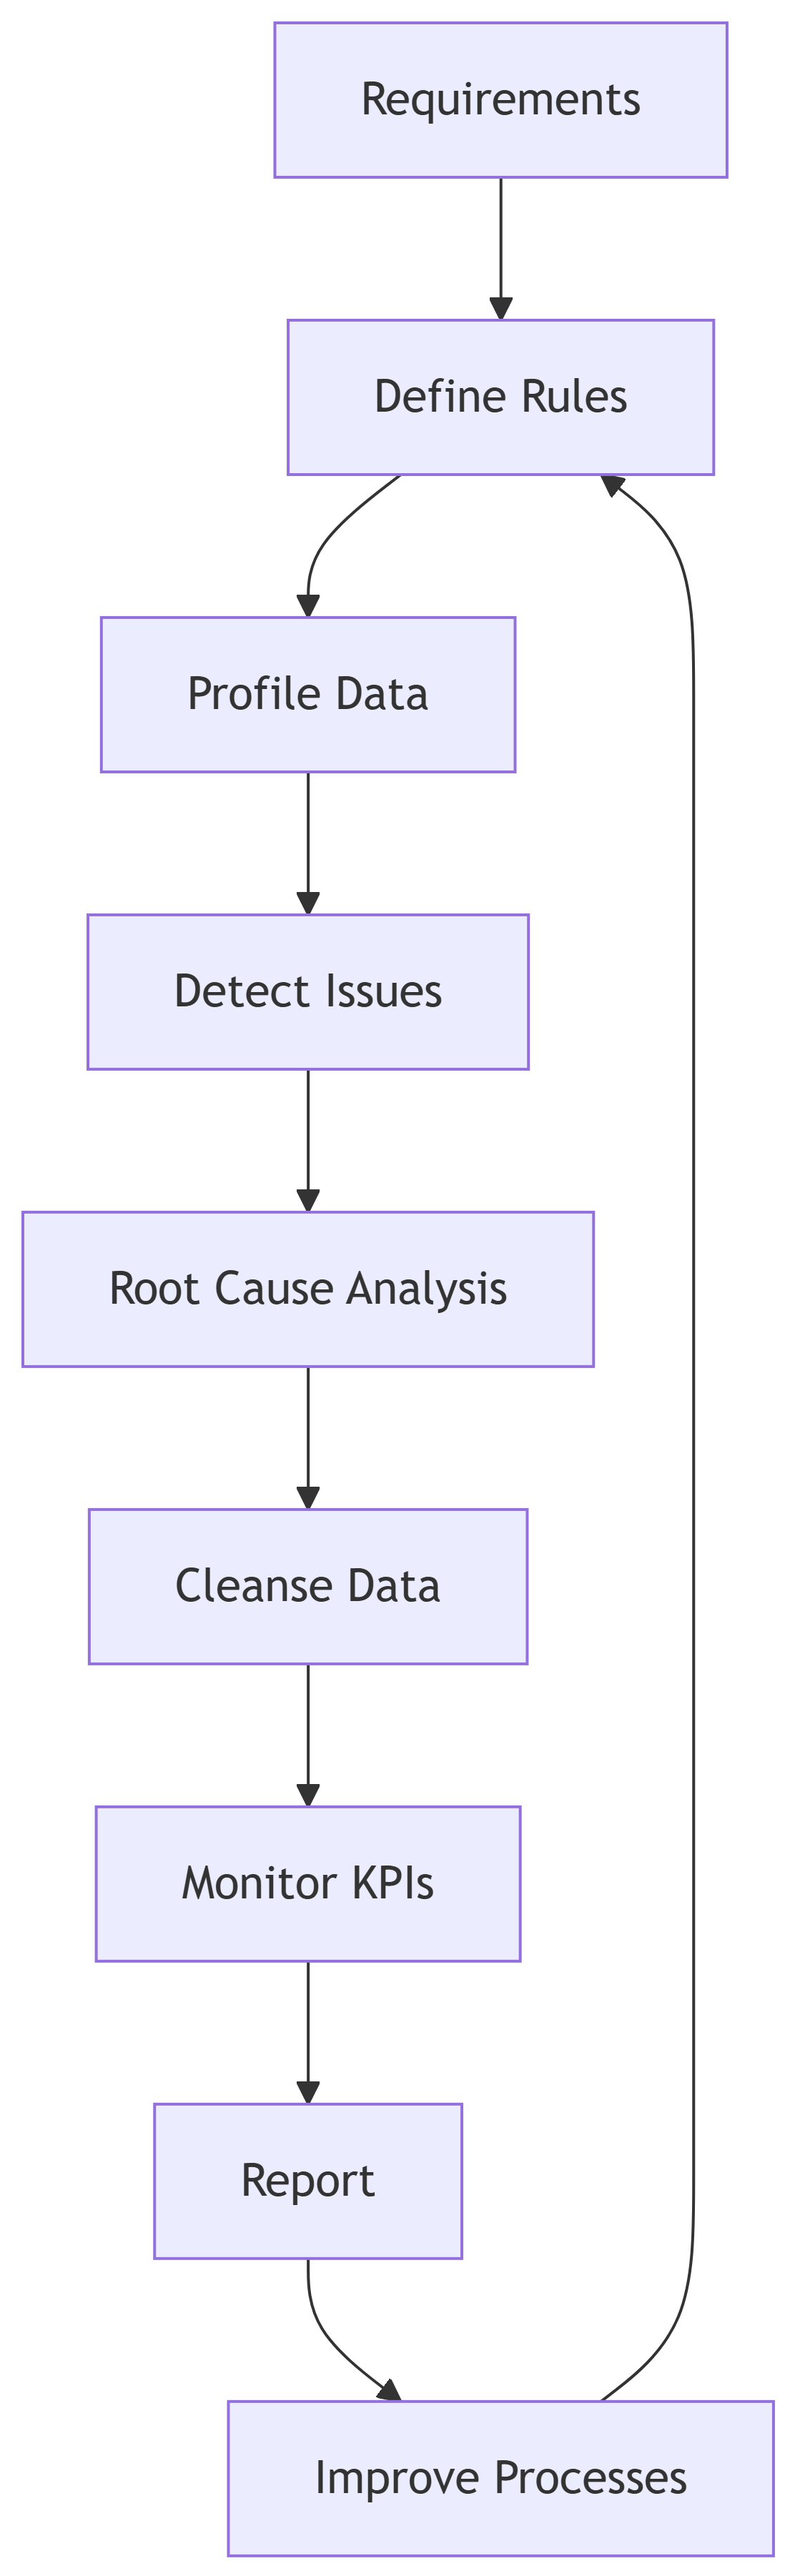
\includegraphics[width=2.9in,height=9.4in]{dama_dmbok_cobit_style_v2_files/figure-latex/mermaid-figure-11.png}

\subsection{10.2 Metadata Management
Flow}\label{metadata-management-flow}

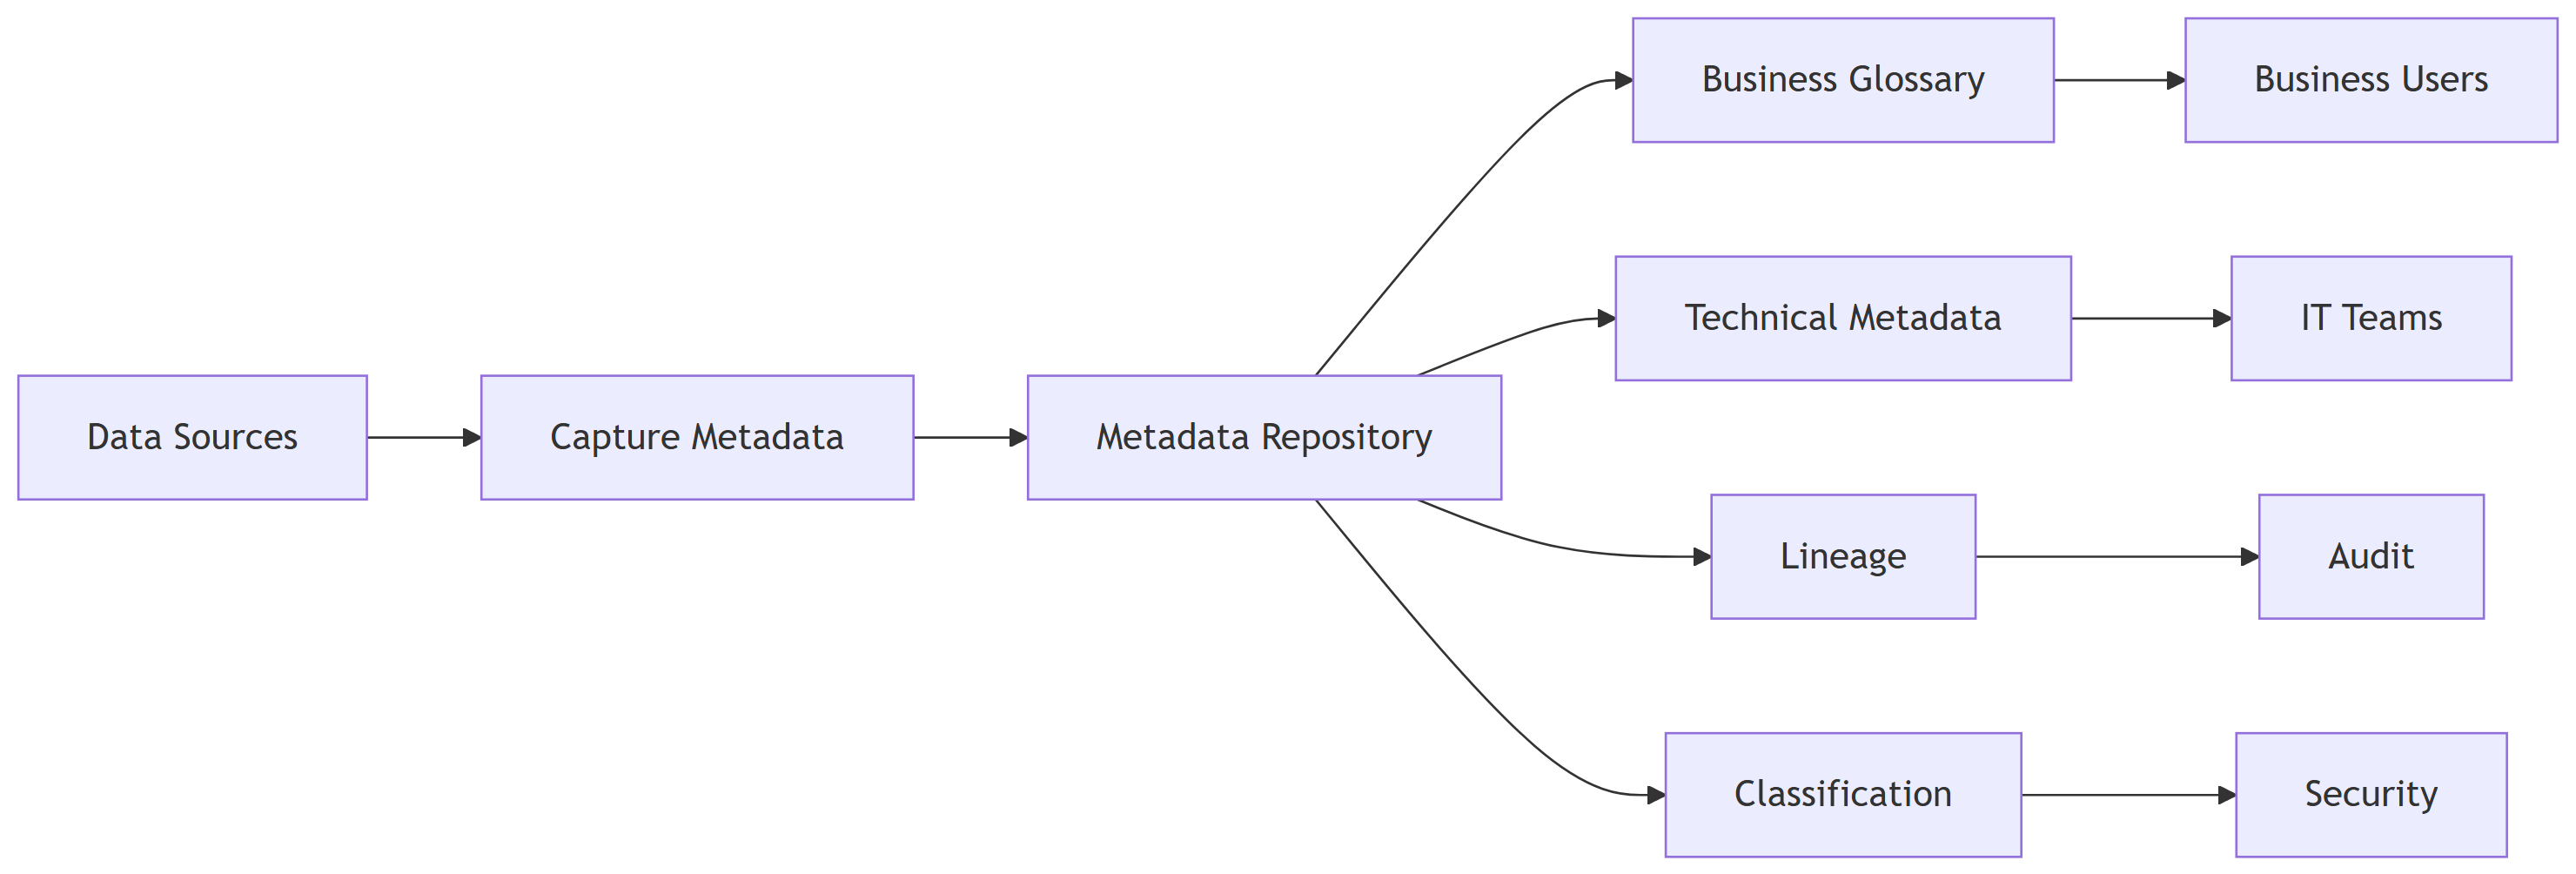
\includegraphics[width=11.71in,height=3.98in]{dama_dmbok_cobit_style_v2_files/figure-latex/mermaid-figure-10.png}

\subsection{10.3 Master Data Management}\label{master-data-management}

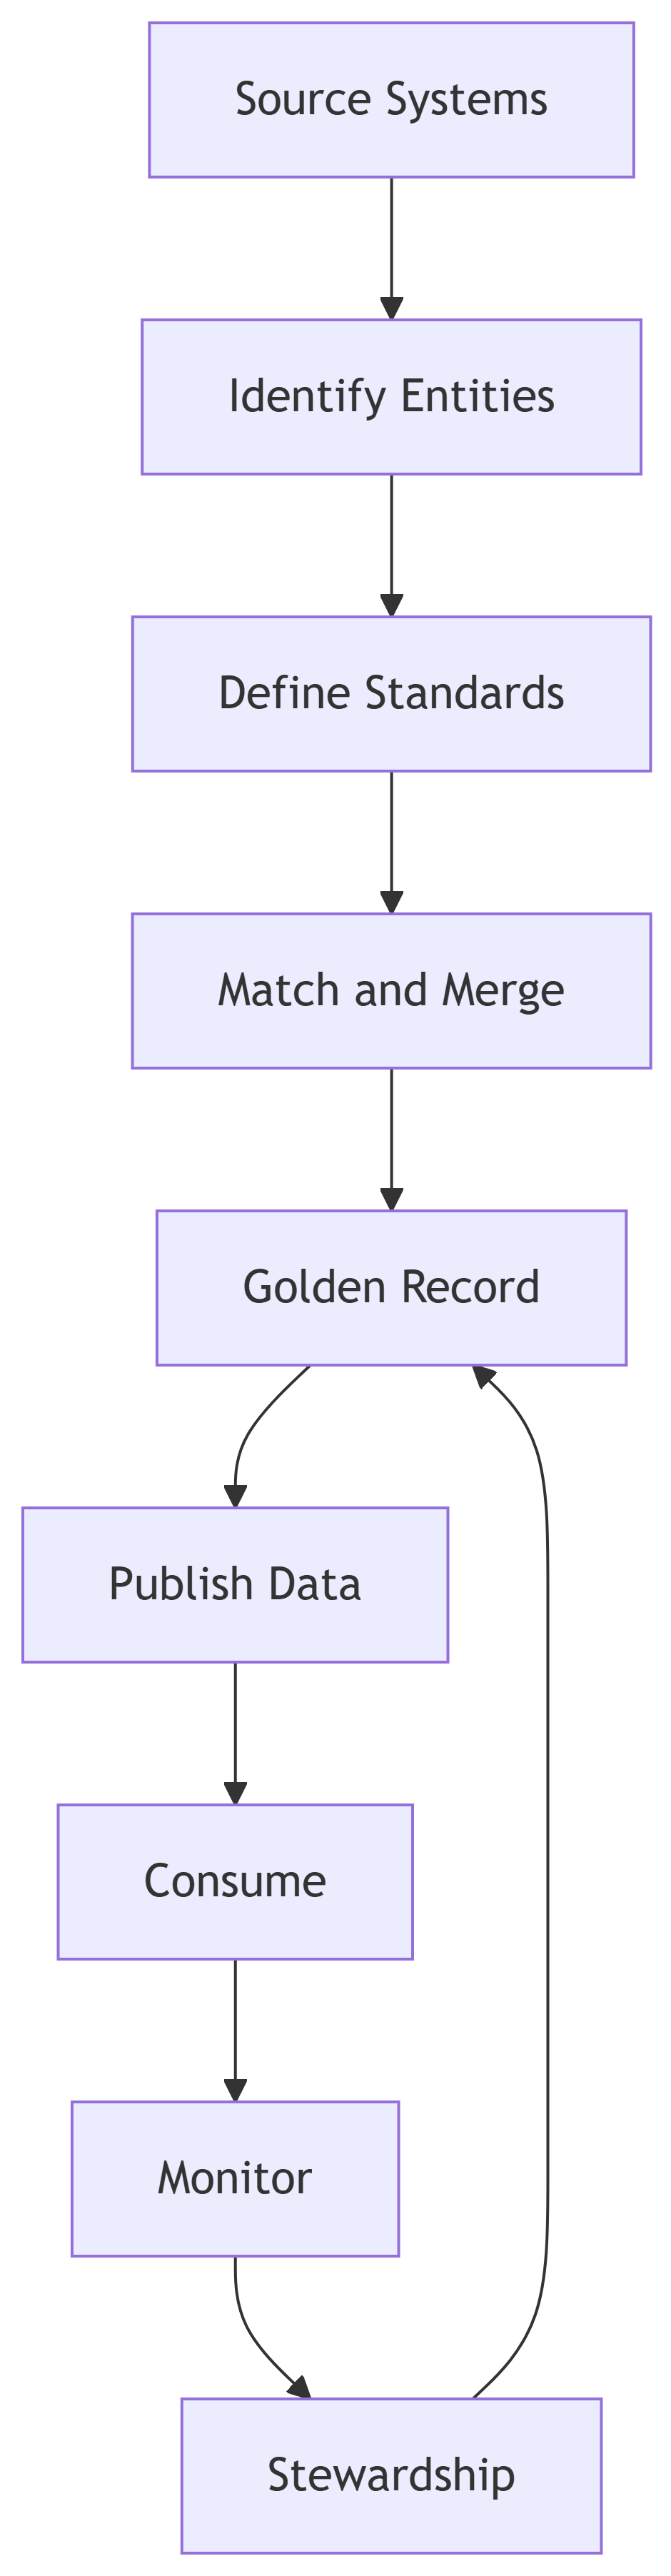
\includegraphics[width=2.46in,height=9.4in]{dama_dmbok_cobit_style_v2_files/figure-latex/mermaid-figure-9.png}

\subsection{10.4 Data Security and
Privacy}\label{data-security-and-privacy}

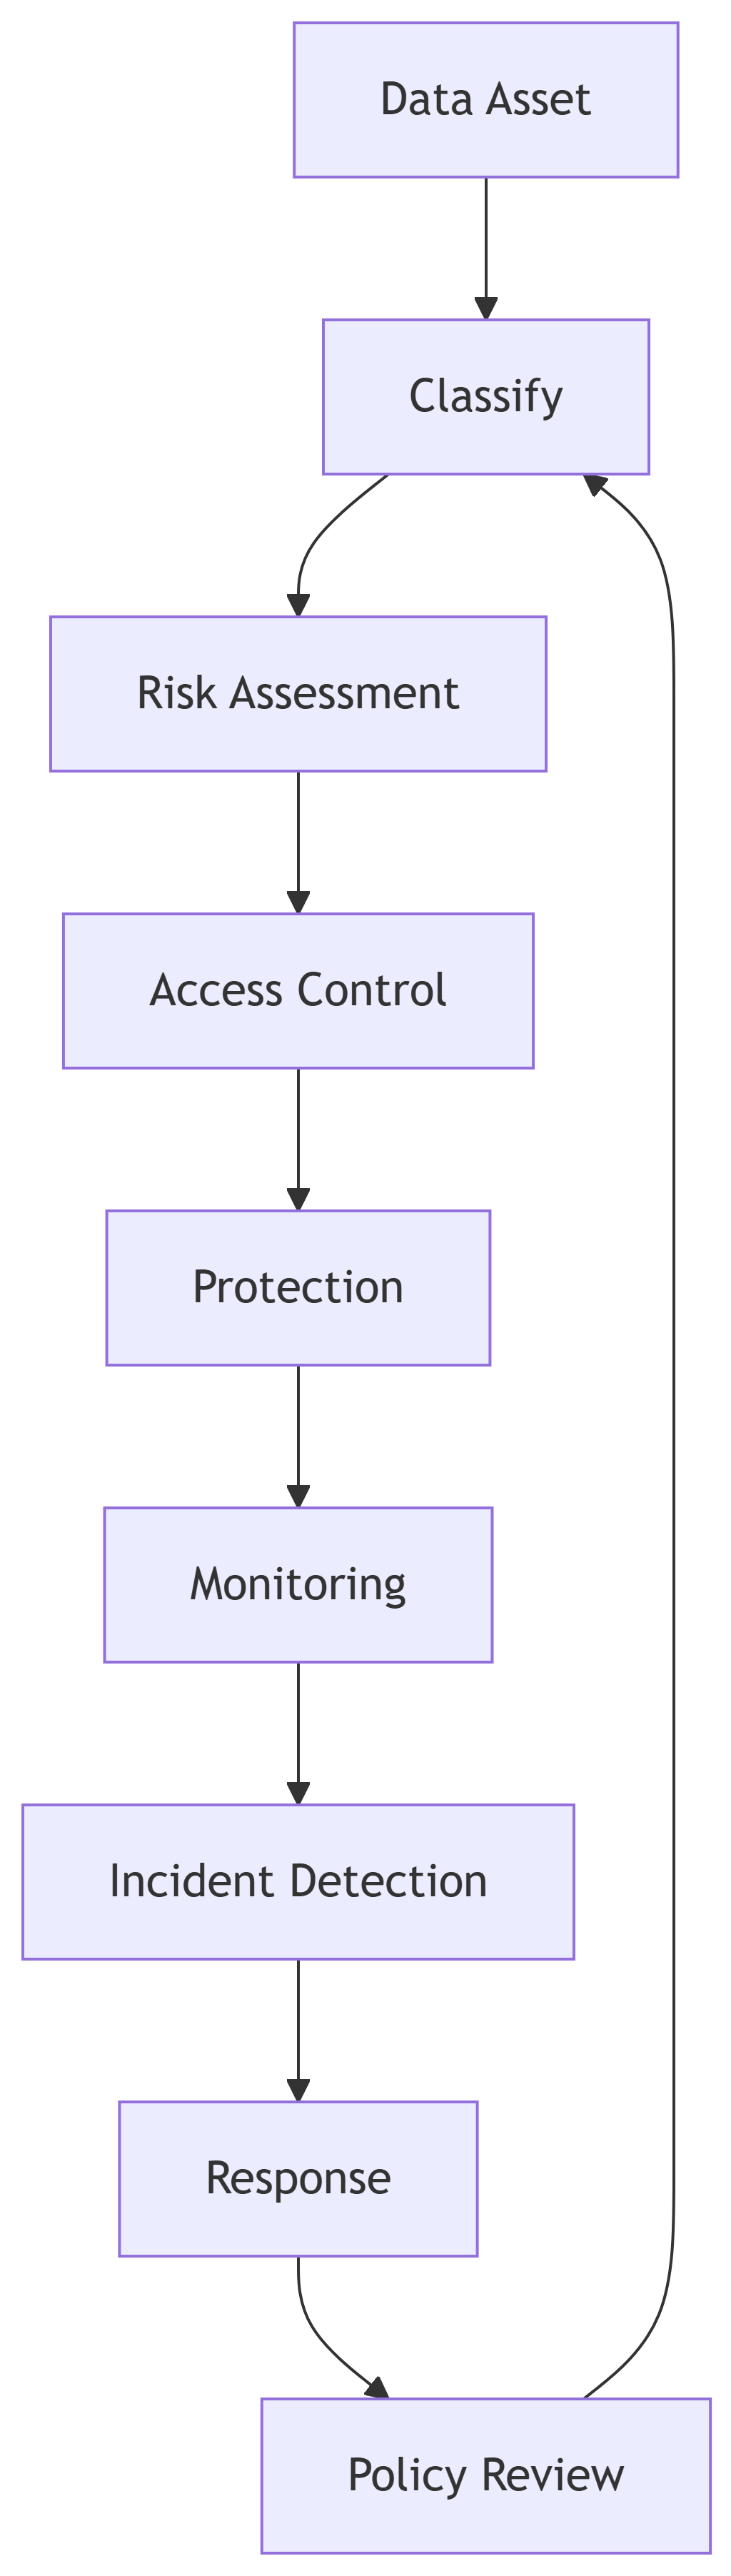
\includegraphics[width=2.67in,height=9.4in]{dama_dmbok_cobit_style_v2_files/figure-latex/mermaid-figure-8.png}

\subsection{10.5 Data Issue Management}\label{data-issue-management}

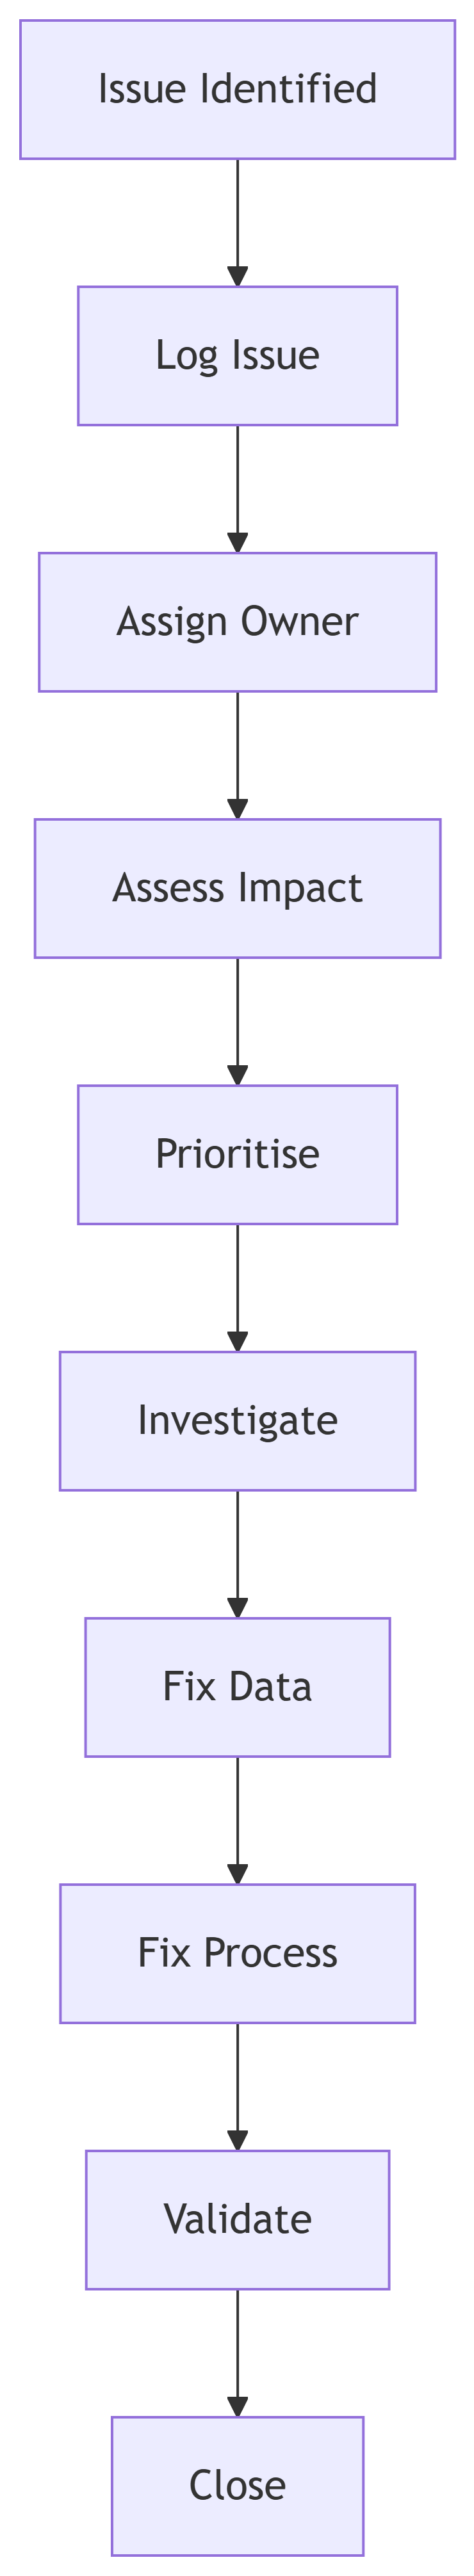
\includegraphics[width=1.93in,height=10.48in]{dama_dmbok_cobit_style_v2_files/figure-latex/mermaid-figure-7.png}

\section{11. Integration with Other
Frameworks}\label{integration-with-other-frameworks}

\subsection{11.1 DMBOK and COBIT}\label{dmbok-and-cobit}

\begin{longtable}[]{@{}ll@{}}
\toprule\noalign{}
DMBOK Area & COBIT Alignment \\
\midrule\noalign{}
\endhead
\bottomrule\noalign{}
\endlastfoot
Data Governance & EDM, APO14 \\
Data Quality & APO11, DSS06 \\
Data Architecture & APO03, BAI03 \\
Data Security & DSS05 \\
Metadata Management & APO03, MEA \\
Master Data & APO14, BAI \\
BI and Analytics & APO, MEA \\
\end{longtable}

\textbf{Interpretation:} COBIT establishes governance expectations and
control objectives. DMBOK provides the data management disciplines
needed to fulfil those expectations.

\subsection{11.2 DMBOK and ITIL}\label{dmbok-and-itil}

\begin{longtable}[]{@{}ll@{}}
\toprule\noalign{}
DMBOK Area & ITIL Alignment \\
\midrule\noalign{}
\endhead
\bottomrule\noalign{}
\endlastfoot
Data Quality & Continual Improvement \\
Metadata Management & Knowledge Management \\
Data Security & Information Security Management \\
Data Storage and Operations & Service Operation \\
BI and Analytics & Measurement and Reporting \\
Master Data & Service Configuration and operational data use \\
\end{longtable}

\subsection{11.3 DMBOK and TOGAF}\label{dmbok-and-togaf}

\begin{longtable}[]{@{}ll@{}}
\toprule\noalign{}
DMBOK Area & TOGAF Alignment \\
\midrule\noalign{}
\endhead
\bottomrule\noalign{}
\endlastfoot
Data Architecture & Data Architecture \\
Data Modelling and Design & Architecture development detail \\
Metadata Management & Architecture repository and content \\
Integration and Interoperability & Application and data architecture \\
Governance & Architecture governance \\
\end{longtable}

\subsection{11.4 Cross-Framework
Positioning}\label{cross-framework-positioning}

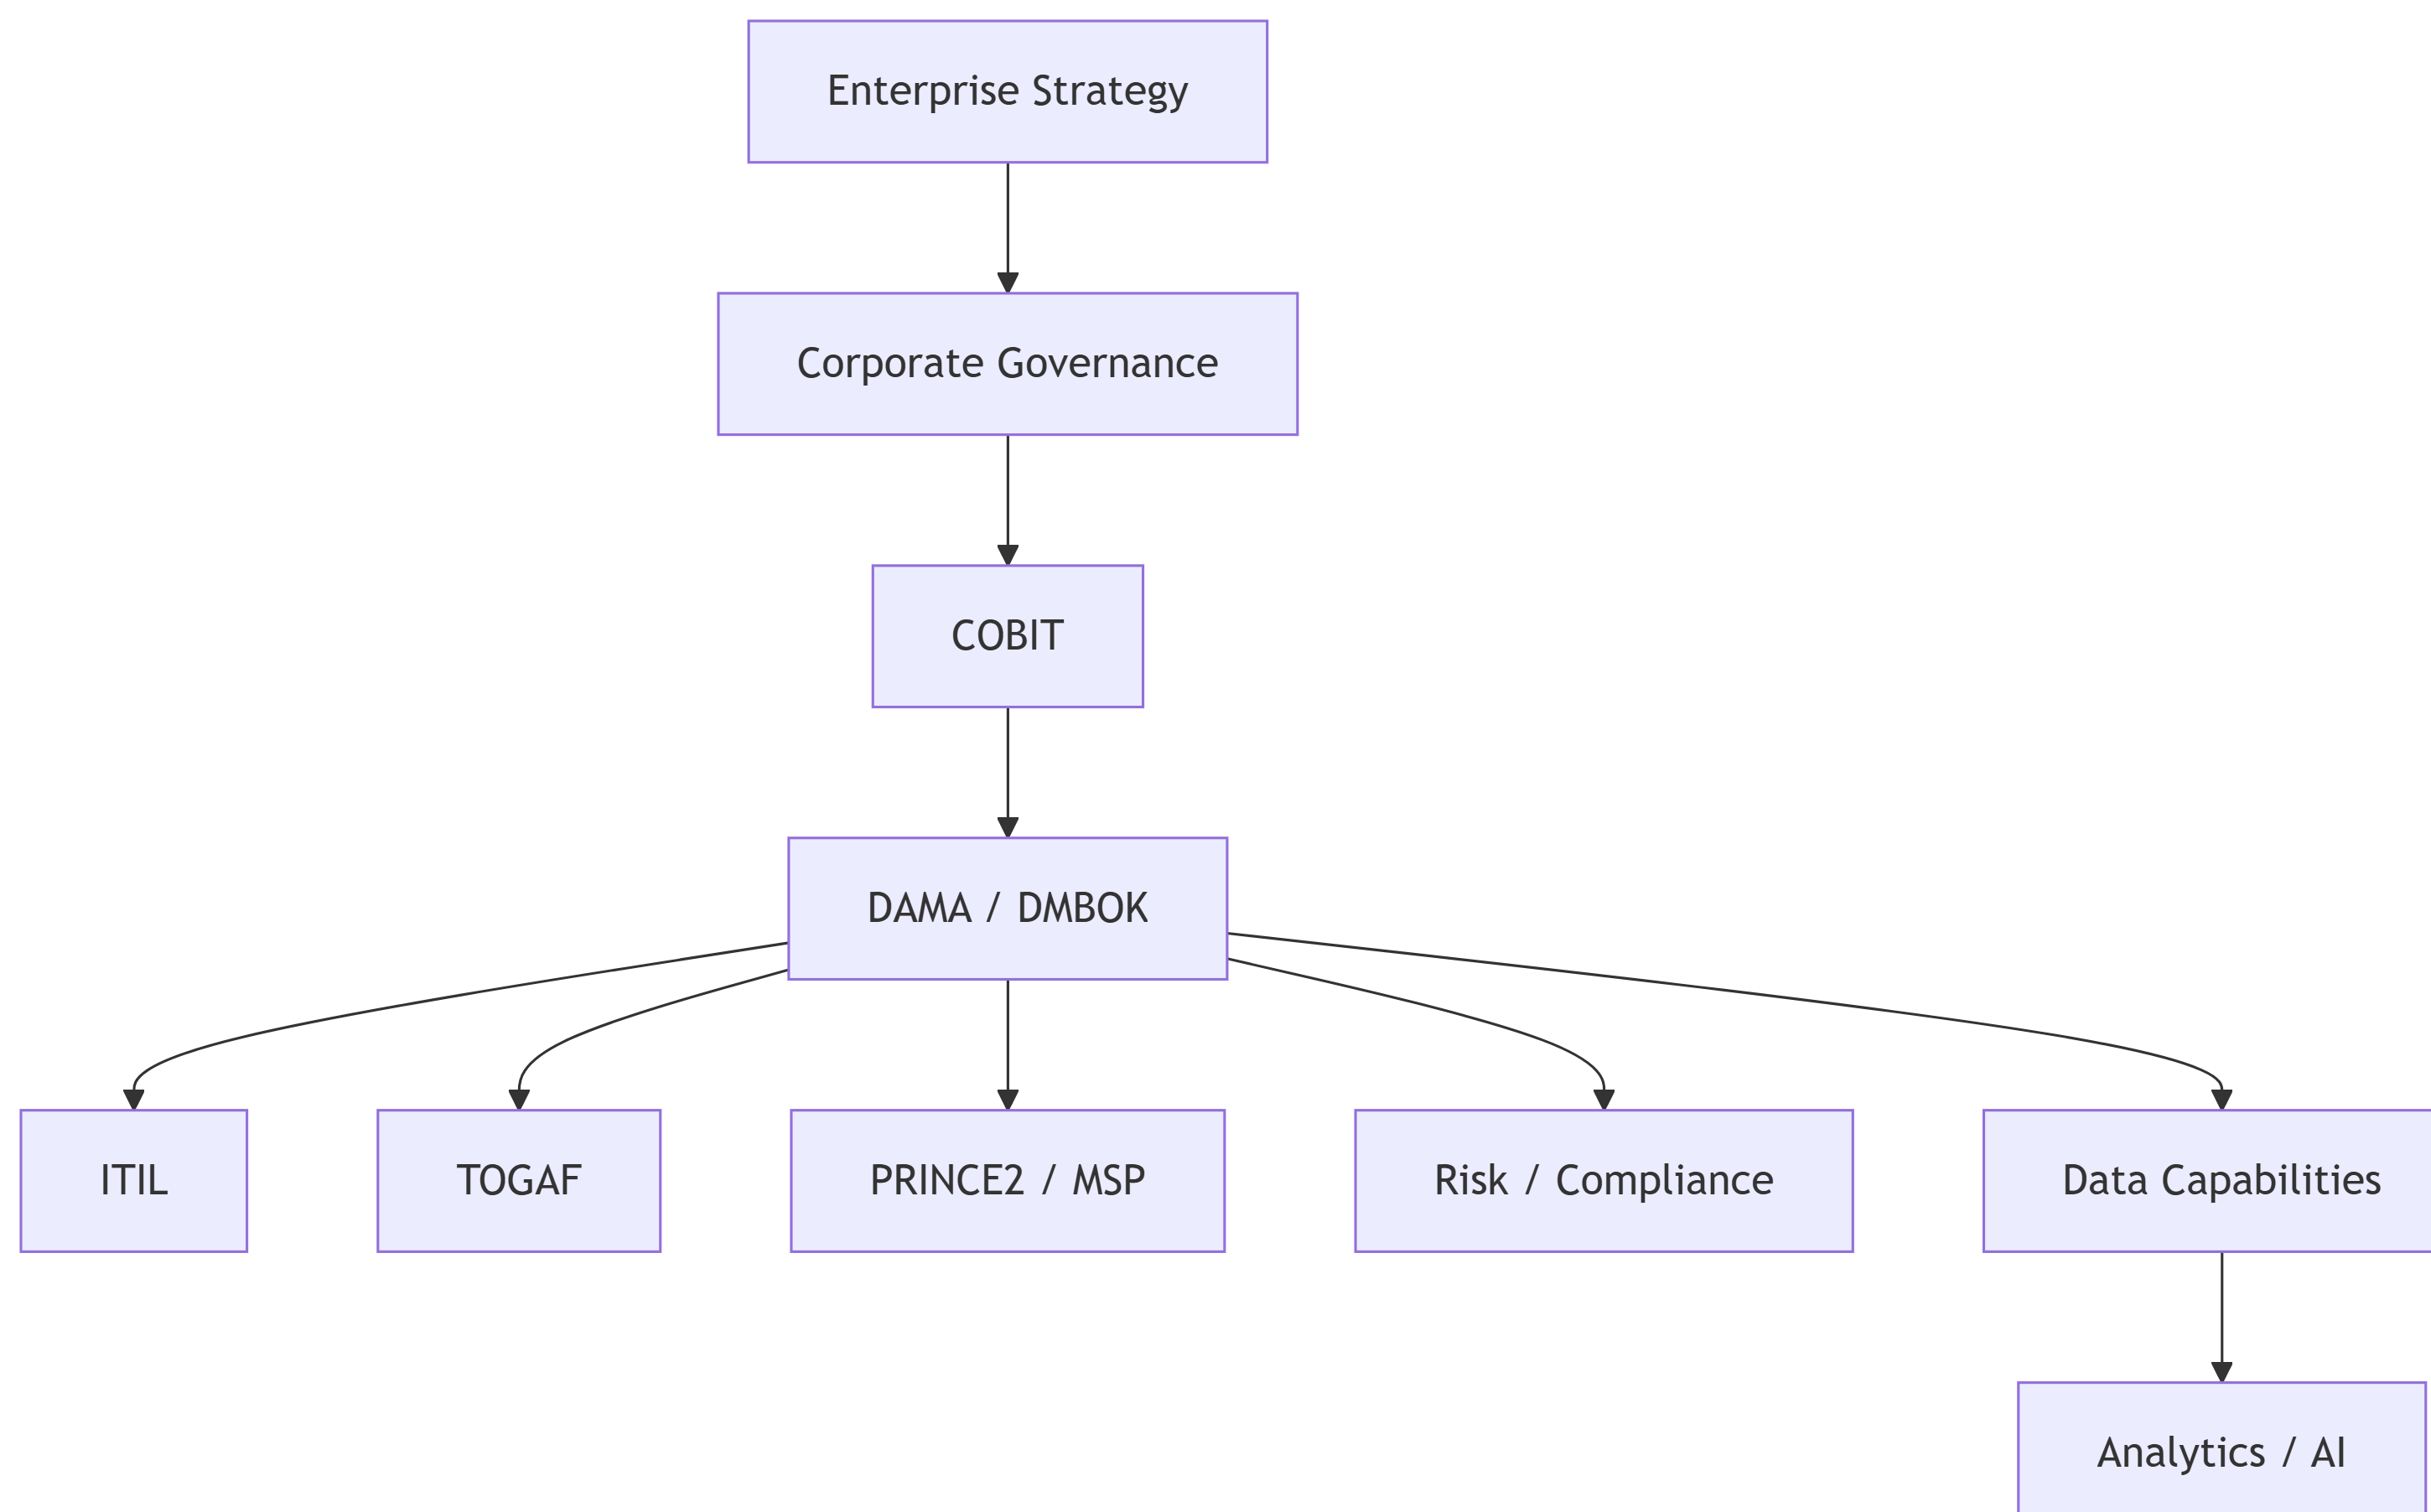
\includegraphics[width=9.87in,height=6.15in]{dama_dmbok_cobit_style_v2_files/figure-latex/mermaid-figure-6.png}

\section{12. Capability Maturity View}\label{capability-maturity-view}

\subsection{12.1 Maturity Progression}\label{maturity-progression}

\begin{longtable}[]{@{}ll@{}}
\toprule\noalign{}
Level & Description \\
\midrule\noalign{}
\endhead
\bottomrule\noalign{}
\endlastfoot
0 & No meaningful data management discipline \\
1 & Ad hoc and reactive practices \\
2 & Repeatable local practices \\
3 & Defined enterprise practices \\
4 & Managed and measured capabilities \\
5 & Optimised, trusted, and data-driven enterprise \\
\end{longtable}

\subsection{12.2 Maturity Journey}\label{maturity-journey}

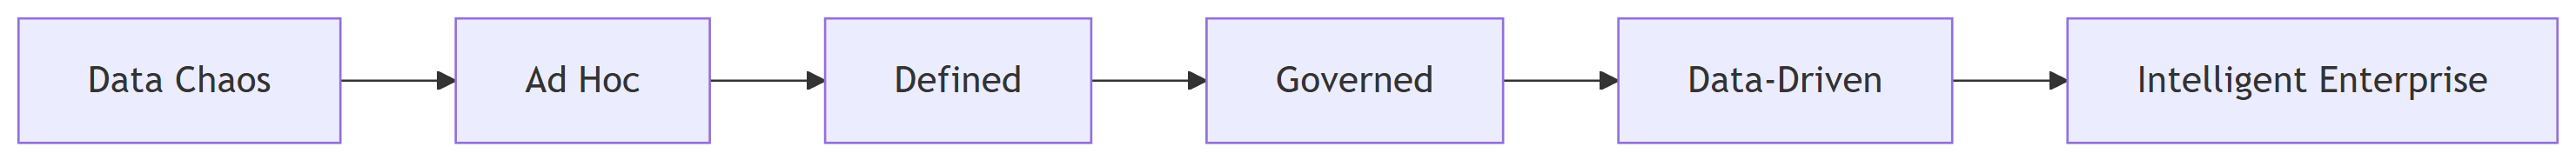
\includegraphics[width=11.63in,height=0.73in]{dama_dmbok_cobit_style_v2_files/figure-latex/mermaid-figure-5.png}

\section{13. Implementation Approach}\label{implementation-approach}

\subsection{13.1 Practical Implementation
Path}\label{practical-implementation-path}

\begin{enumerate}
\def\labelenumi{\arabic{enumi}.}
\tightlist
\item
  Assess current-state maturity and pain points.
\item
  Define enterprise data strategy and principles.
\item
  Establish governance roles, councils, ownership, and stewardship.
\item
  Prioritise critical data domains and use cases.
\item
  Implement foundational capabilities such as metadata, quality, and
  master data.
\item
  Strengthen security, privacy, and retention controls.
\item
  Enable reporting, analytics, and insight generation.
\item
  Monitor outcomes and improve continuously.
\end{enumerate}

\subsection{13.2 Typical Early
Priorities}\label{typical-early-priorities}

\begin{itemize}
\tightlist
\item
  data ownership and stewardship
\item
  business glossary and metadata catalogue
\item
  critical data quality rules
\item
  master data for key entities
\item
  privacy and classification controls
\item
  lineage for high-risk or high-value data flows
\end{itemize}

\section{14. KPIs and Measures}\label{kpis-and-measures}

\begin{longtable}[]{@{}ll@{}}
\toprule\noalign{}
Area & Example KPI \\
\midrule\noalign{}
\endhead
\bottomrule\noalign{}
\endlastfoot
Data Quality & \% completeness, \% accuracy, defect rate \\
Metadata & \% of critical data assets documented \\
Governance & Policy compliance rate, ownership coverage \\
Security & Number of data incidents, access control exceptions \\
Master Data & Duplicate rate, mastered entity coverage \\
BI and Analytics & Report adoption, trusted data source usage \\
Issue Management & Time to resolve data issues \\
\end{longtable}

\section{15. Strengths and Limitations}\label{strengths-and-limitations}

\subsection{15.1 Strengths}\label{strengths}

\begin{itemize}
\tightlist
\item
  broad and coherent coverage of data management disciplines
\item
  suitable for enterprise-wide operating models
\item
  strong bridge between business and technology
\item
  useful foundation for data governance and analytics programmes
\item
  flexible enough to be adapted to different sectors and maturity levels
\end{itemize}

\subsection{15.2 Limitations}\label{limitations}

\begin{itemize}
\tightlist
\item
  not a prescriptive implementation method
\item
  requires tailoring to become operational
\item
  can feel broad or abstract without a clear delivery model
\item
  works best when integrated with governance, architecture, service,
  risk, and change frameworks
\end{itemize}

\section{16. When to Use DMBOK}\label{when-to-use-dmbok}

DMBOK is especially useful when an organisation needs to:

\begin{itemize}
\tightlist
\item
  establish or refresh enterprise data governance
\item
  improve data quality and trust
\item
  create a business glossary and metadata capability
\item
  define master data ownership and control
\item
  connect data governance with architecture and service management
\item
  support regulatory, audit, and assurance needs around data
\item
  strengthen the data foundations for AI, analytics, and automation
\end{itemize}

\section{17. Position in the Enterprise Governance
Model}\label{position-in-the-enterprise-governance-model}

\subsection{17.1 Enterprise Data Capability
Map}\label{enterprise-data-capability-map}

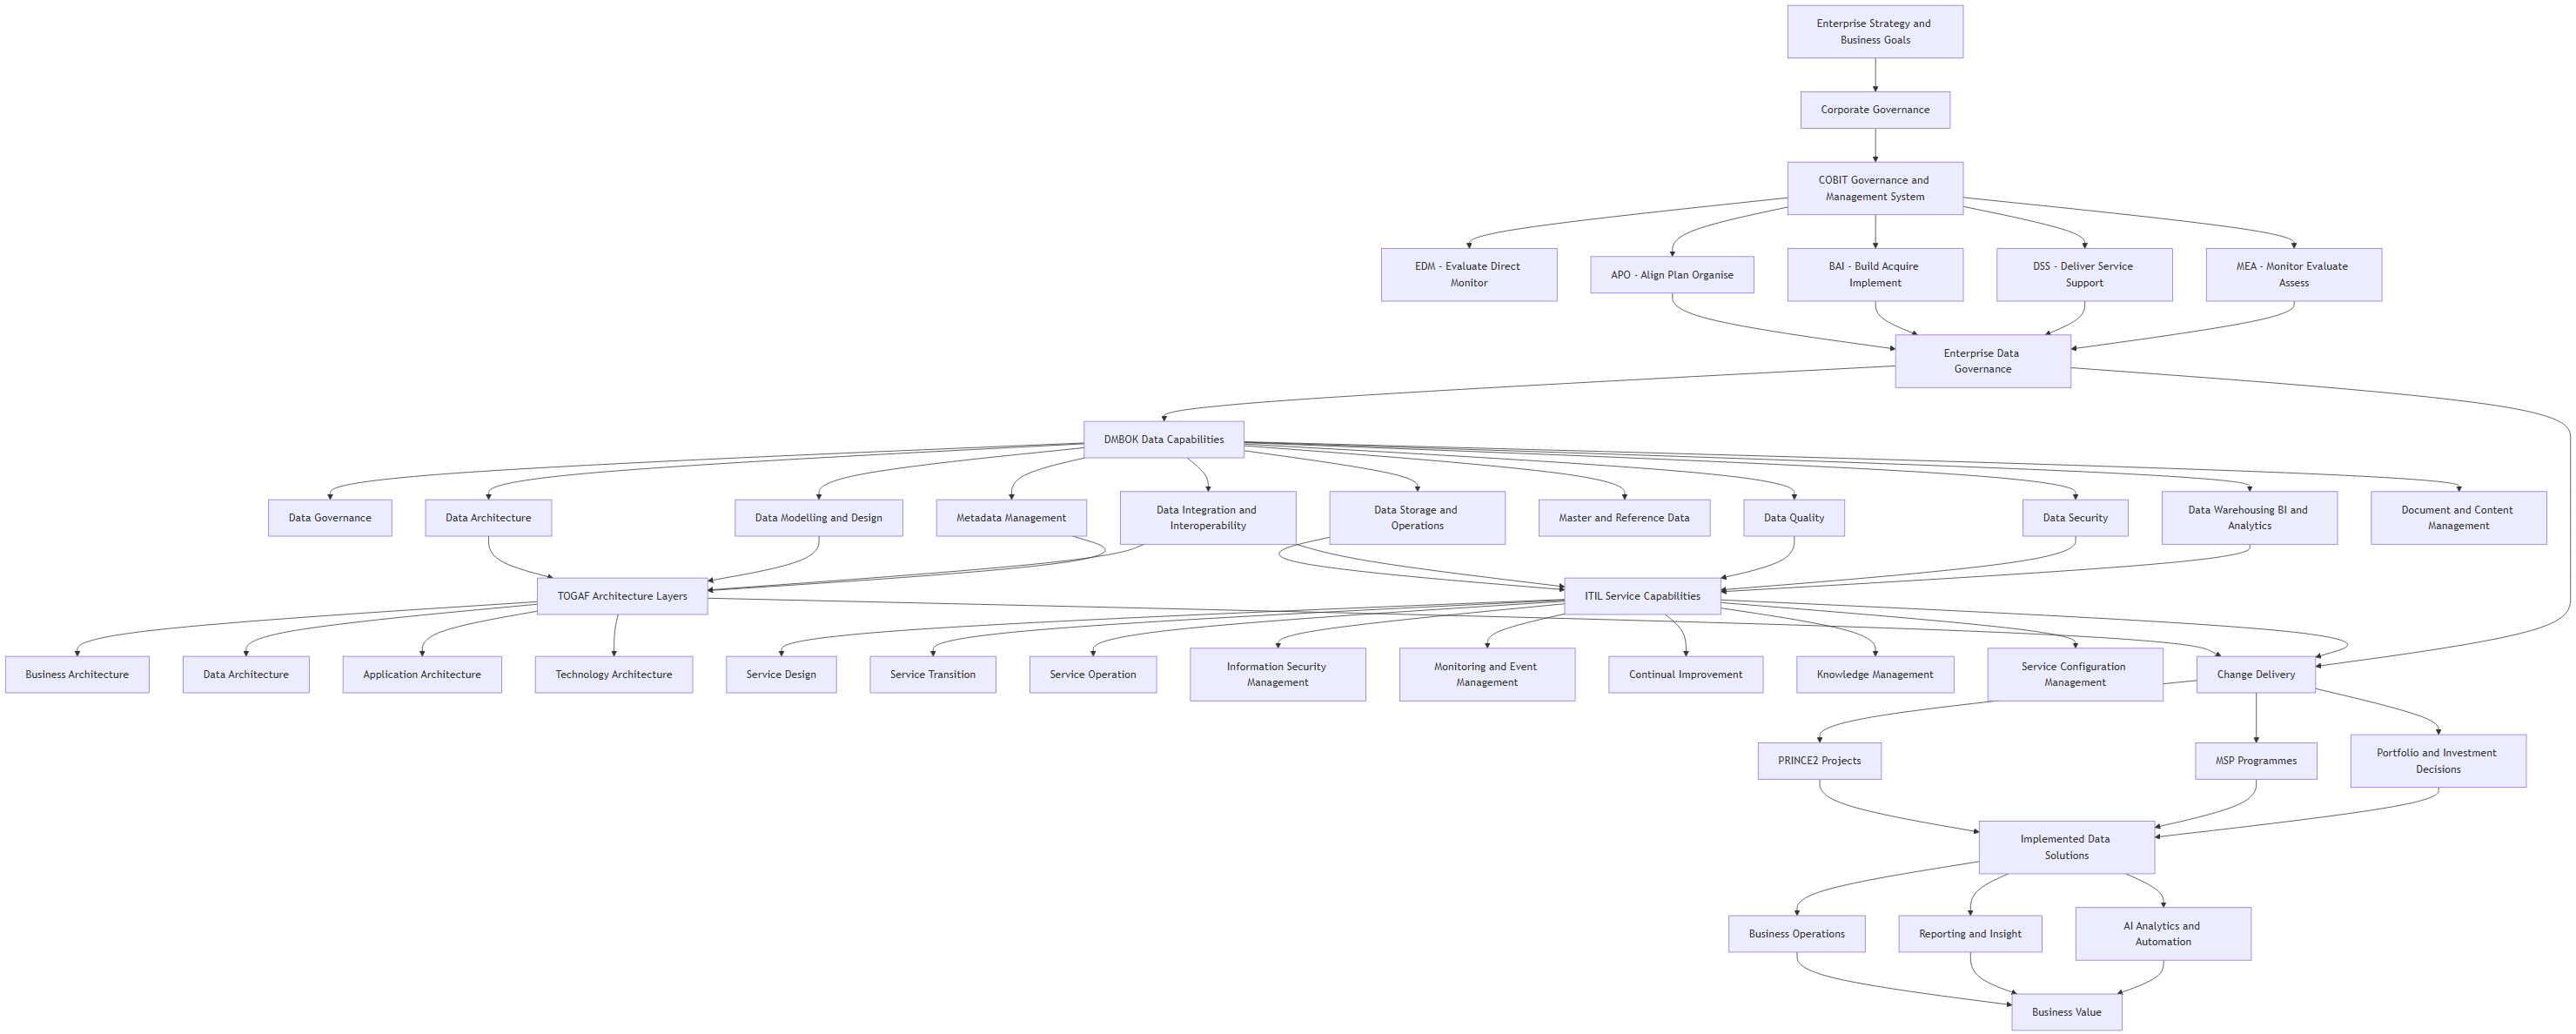
\includegraphics[width=39.74in,height=15.98in]{dama_dmbok_cobit_style_v2_files/figure-latex/mermaid-figure-4.png}

\subsection{17.2 Positioning Statement}\label{positioning-statement}

Within the broader enterprise governance model, COBIT provides the
governance shell, DMBOK provides the data capability model, TOGAF
provides architectural structure, ITIL provides operational service
management, and PRINCE2 or MSP provide delivery mechanisms for change.

\section{18. Visual Governance Atlas
Additions}\label{visual-governance-atlas-additions}

\subsection{18.1 Cross-Framework Document
Flow}\label{cross-framework-document-flow}

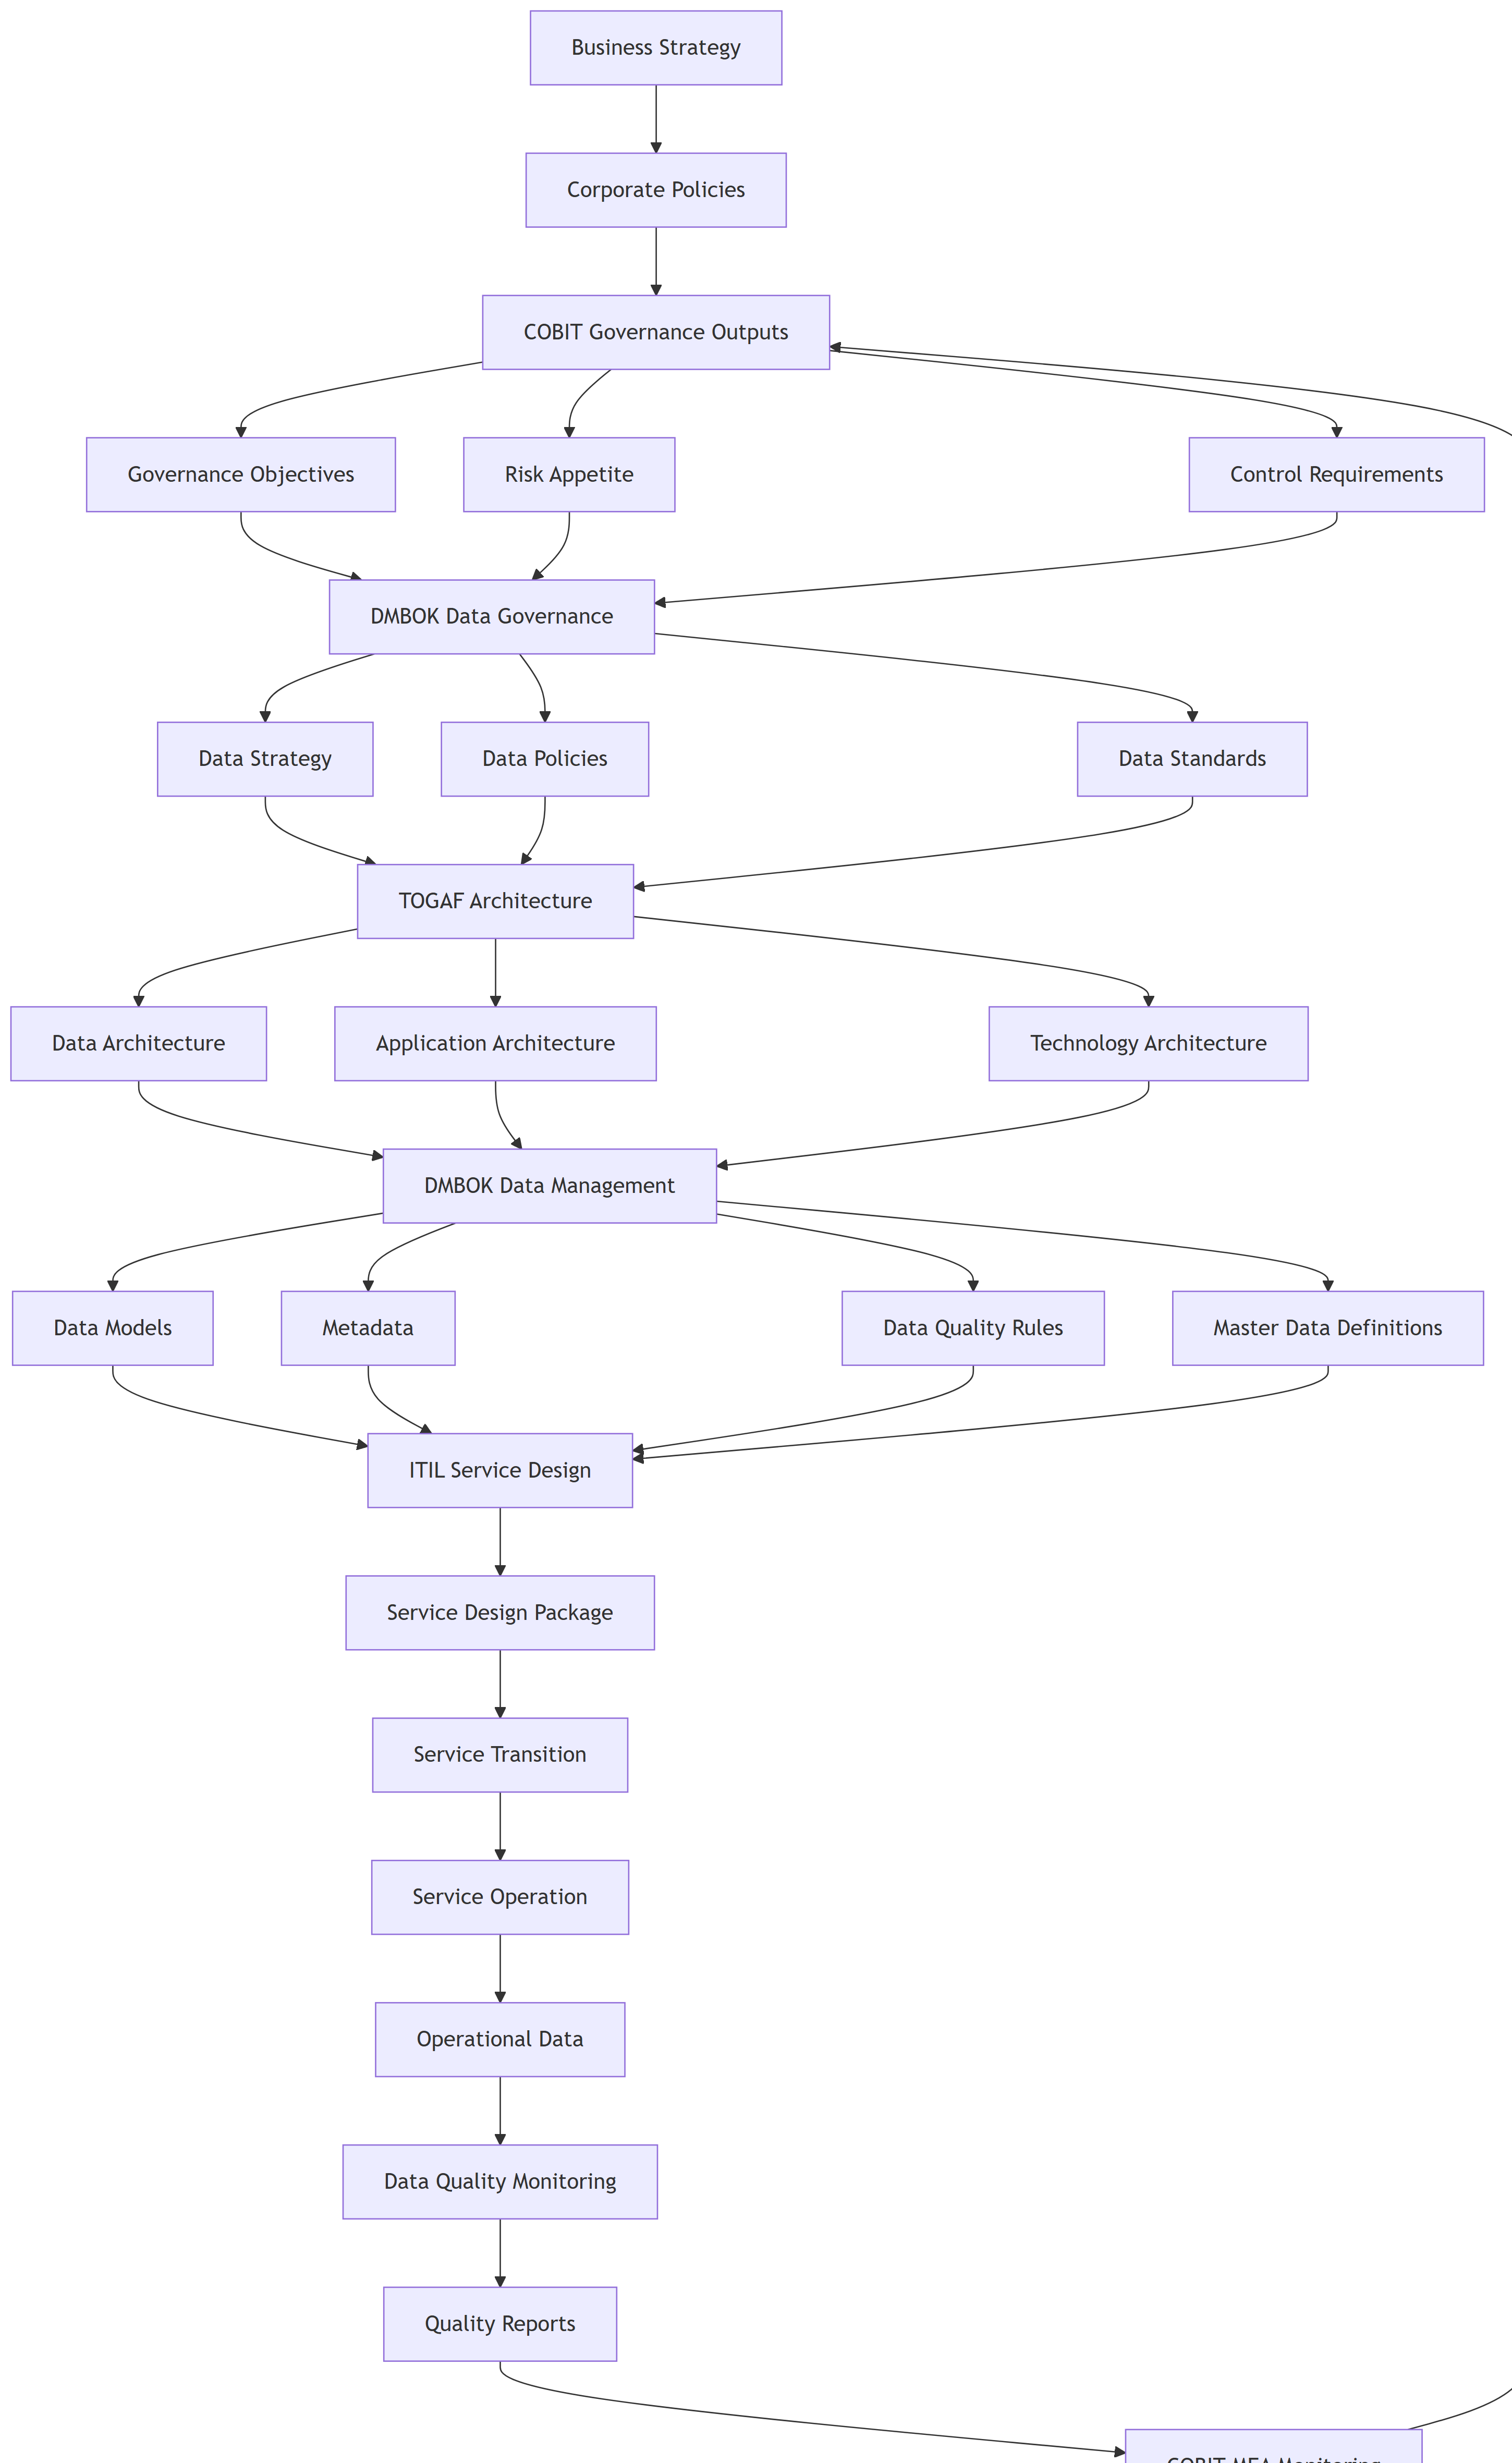
\includegraphics[width=11.75in,height=19.15in]{dama_dmbok_cobit_style_v2_files/figure-latex/mermaid-figure-3.png}

\subsection{18.2 Unified Enterprise Governance
Meta-Model}\label{unified-enterprise-governance-meta-model}

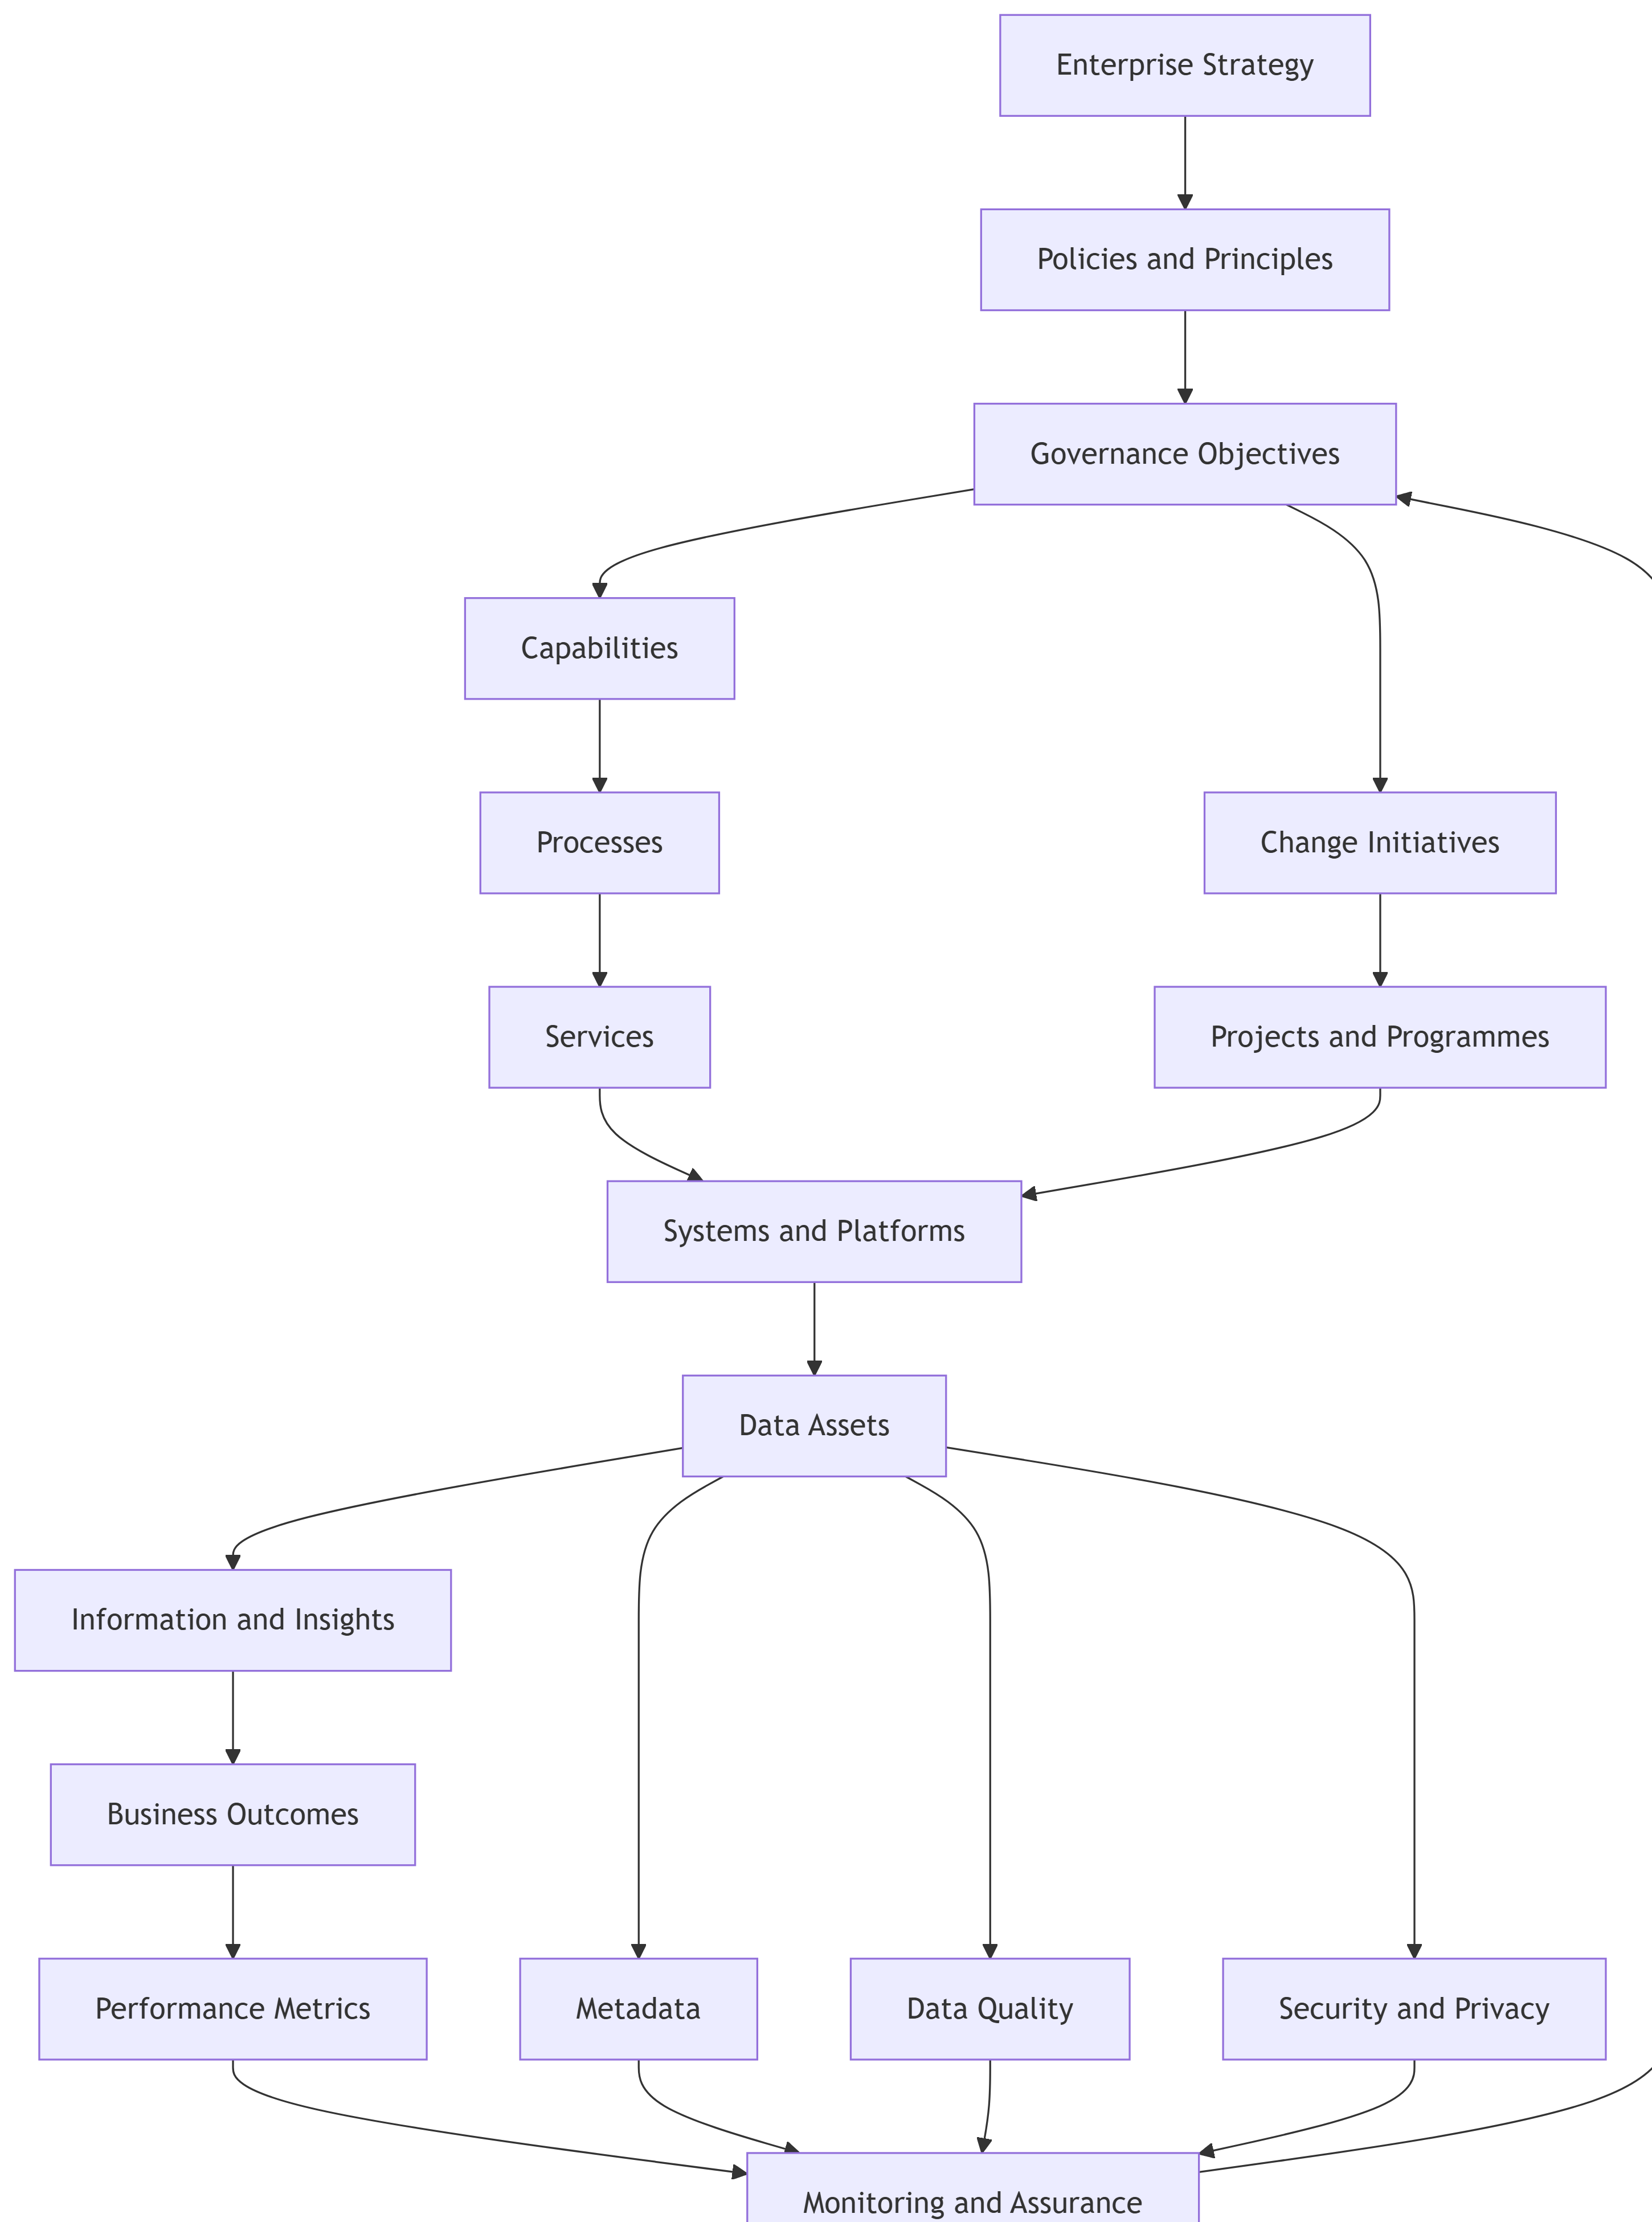
\includegraphics[width=9.4in,height=12.65in]{dama_dmbok_cobit_style_v2_files/figure-latex/mermaid-figure-2.png}

\section{19. Key Takeaways}\label{key-takeaways}

\begin{itemize}
\tightlist
\item
  DAMA provides the organisational and professional context.
\item
  DMBOK provides the structured body of knowledge for enterprise data
  management.
\item
  DMBOK is strongest when used as part of an integrated governance model
  rather than as a standalone data initiative.
\item
  Metadata, quality, security, and stewardship are foundational to
  sustainable data governance.
\item
  Documents and artefacts are the practical integration layer between
  DMBOK and the wider framework landscape.
\item
  DMBOK is a strong bridge between governance intent and operational
  data capability.
\end{itemize}

\section{20. References}\label{references}

\begin{itemize}
\tightlist
\item
  DAMA International -- Data Management Body of Knowledge
\item
  DAMA International -- CDMP Certification
\item
  Enterprise good practice in data governance, data management, and data
  architecture
\end{itemize}




\end{document}
